%------------------------------------------------
% Contains the actual report content
%
% Author: Jérémy Singy
%------------------------------------------------

% Define a nice-looking C# logo for the text
\newcommand{\Csh}{C$^\sharp$}

% Chapters content

\chapter{Introduction}

\section{Context}

For several years, Carl Haber and his team at Lawrence Berkeley National Laboratory (\gls{lbnl}) have been working on the sound recovery of old mechanical records. They developed systems able to recover the sound from mediums using optical technologies, without any physical contact. These solutions are able to process many different record types, from early Edison cylinders to vinyl discs, including shellac or lacquer composed discs and others.

Nowadays, a lot of unique records remain in archives stored in different libraries, museums and academic institutions, containing materials of important historical and cultural value. Since most of them are recorded on aging and deteriorated mediums, it is often too delicate to play them with a normal mechanical phonograph. Non-contact feature of optical methods is then important.

The team at \gls{lbnl} first started to develop a system called \gls{irene}. It enables to extract the sound using digitized images of a disc. The installation for acquisition is completed by a software package that processes the extraction step, called \gls{rene}. Some time later, the development of a new project called \gls{3dprobe} started. Instead of capturing 2D images, the acquisition uses a special probe able to measure the real depth on the surface of the scanned record. This new system has enabled to process other types of records such as cylinders and is able to offer a better outcome with some specific mediums.

Even earlier in Switzerland, at the College of Engineering and Architecture of Fribourg, another project called VisualAudio has been set up. It aims to archive discs that are deteriorating in a durable way so that the recordings can be heard years later. The discs are stored on a photographic film which is a support with a long life span. An application has also been developed, enabling to extract the sound using non-contact optical scanning in a way similar to \gls{irene}.

\section{Project goals}

Old records can suffer from degradations. One of the most common is known as ``cracked discs''. This problem appears when the lacquer coating shrinks as the disk is getting older. This causes cracks where the underneath hard support is visible, as seen in \autoref{fig:crackeddisc}. Some records are also entirely broken into pieces. The acquisition is then performed in several steps by strapping the pieces together. The result is also some discontinuous grooves between the different pieces.

\begin{figure}[!ht]
\centering
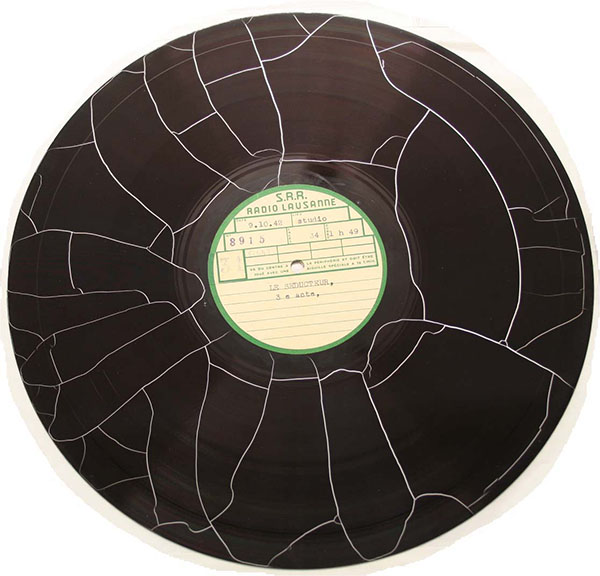
\includegraphics[width=0.7\textwidth]{images/cracked-disc}
\caption{An example of cracked disc.}
\label{fig:crackeddisc}
\end{figure}

Up to now, \gls{irene} and \gls{3dprobe} cannot automatically process such damaged records, because the groove traces are sometimes widely separated and may be shifted from each other. Though a special feature is implemented, enabling the user to manually track the traces, it is not a perfect tool for practical use. Moreover, even with such a feature, it could be really difficult to visually find the correct shifting when the traces look similar.

The aim of this Master's thesis is to find ways to read correctly these kinds of degraded records with the solutions developed at LBNL by Carl Haber and his team. In a first step, an improvement of the manual tracking will be implemented. It is still useful to keep it for some cases, e.g for special early recordings or when a disc is heavily cracked.

Then, the next step will be to design and implement a tracking feature able to process cracked records and link their traces automatically. VisualAudio already implements a feature enabling to track cracked discs in an automatic or semi-automatic way. It can then be taken as an example, though it will obviously not be possible to directly adopt its implementation, as the systems are quite different.

\section{Report structure}

This report is separated into three main sections. The first one corresponds to the analysis performed in order to have a good understanding of the subject before starting on the actual project. \ref{chap:phonorecords} details the important points to know about phonograph records, history as well as main techniques implemented between the 19th and the 20th century. Then, \ref{chap:acqprocsys} will presents the current solutions developed at \gls{lbnl}. Both the 2D and 3D acquisition systems will be presented, as well as the processing part involving the different softwares.

The second part will present the main work realized during the thesis. \ref{chap:mantrack} will detail the improvements to help the user for the restoration of profoundly damaged records, using a manual solution. Then, a proposition able to automatically process damaged records in certain circumstances while be presented. The implementation of the different parts is separated from Chapters~\ref{chap:groovedetect} through \ref{chap:linking}.

%TODO end the structure

\chapter{Phonograph cylinders and records}
\label{chap:phonorecords}

This chapter will give a quick historical overview of the different mechanical phonograph technologies and the types of mediums encountered. It will also explain the main principles behind the analog recording

\section{History}

The first known sound recording was realized by the French printer Édouard-Léon Scott de Martinville in 1860. However, the used device called the \emph{phonautograph} was not able to playback the recordings. It rather acted as an early mechanical oscilloscope and was later used by scientists to study visual representations of the sound.

The phonograph was created by Thomas Edison in 1877. It was the first device able to record \emph{and} reproduce the sound. The general principle was to mechanically engrave the audio signal on a rotating cylinder. The resulting groove undulated then vertically. Then, for the playback, a stylus (needle) retraced the groove and was able to reproduce the sound waves from the generated vibrations. Finally, the signal was efficiently coupled to the room environment with a horn so that the recording was more audible. A newer version of this phonograph and an example of cylinder are presented in \autoref{fig:edisonphonocyl}.

\begin{figure}[!ht]
    \begin{subfigure}[b]{0.45\textwidth}
    \centering
    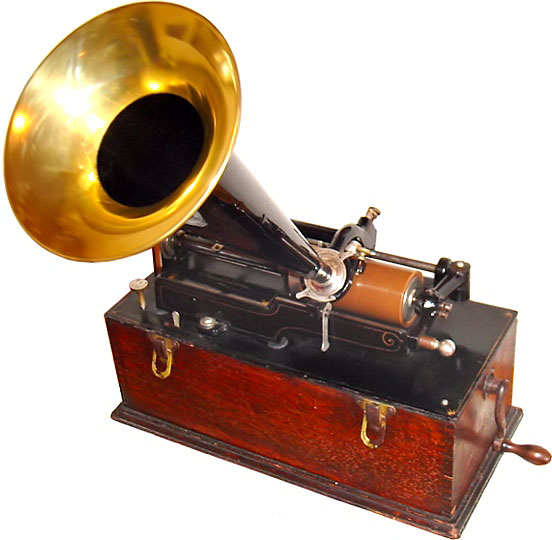
\includegraphics[width=0.8\textwidth]{images/edison-phonograph}
    \caption{An Edison phonograph.}
    \label{fig:edisonphono}
    \end{subfigure}
    \begin{subfigure}[b]{0.45\textwidth}
    \centering
    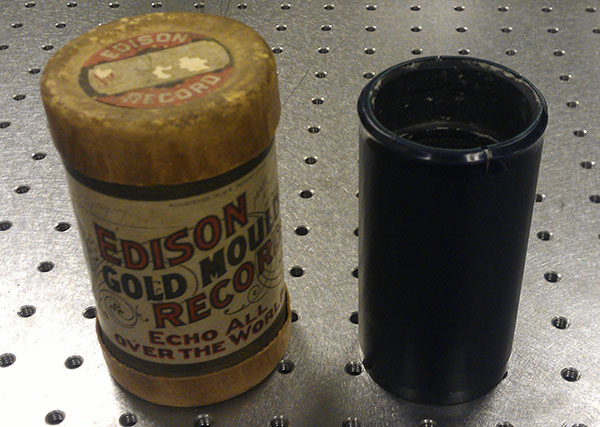
\includegraphics[width=0.9\textwidth]{images/edison-cylinder}
    \caption{An Edison wax-cylinder.}
    \label{fig:edisoncyl}
    \end{subfigure}
    \caption{Pictures of Edison wax phonograph and record.}
    \label{fig:edisonphonocyl}
    %\floatfoot{Norman Bruderhofer, www.cylinder.de}
\end{figure}

Since then, the phonograph has been used as the primary device for sound reproduction until around the 1950's when the magnetic tape became widely available. From the Edison's first version, a lot of improvements have been made. Edison used first a tinfoil around the cylinders into which the groove was embossed. However, this material gave bad quality and was rapidly degrading. Alexander Graham Bell started to use wax-coated cylinders and discs instead of the tinfoil, which improved a lot the sound quality.

Then, in the early twentieth century, the cylinders were gradually replaced by the gramophone records which were flat discs that could be double-sided. On the latter, the groove undulated laterally instead of vertically.

After the wax-cylinders, a lot of different materials have been used for the discs covering. For example, the shellac discs became the first widely used medium. Some discs were also using a special lacquer coat. Finally, the vinyl disc is one of the last types of gramophone record and is still being used today. The different existing recording types will be further explained in \autoref{sec:rectypes}

\section{Basic principle}

\subsection{Edison phonograph}

With the early Edison phonograph, the same device was used to record and play the sound. As already explained, the sound is mechanically embossed with a needle on a tinfoil placed around the cylinder. In fact, the needle is connected to a diaphragm that vibrates when audio waves are emitted. The cylinder is put on a mechanism which can be rotated by a crank and that shifts slowly resulting in helical grooves. To improve acoustic match, a horn (tube) is used, as represented in \autoref{fig:phonoschema}.

\begin{figure}[!ht]
\centering
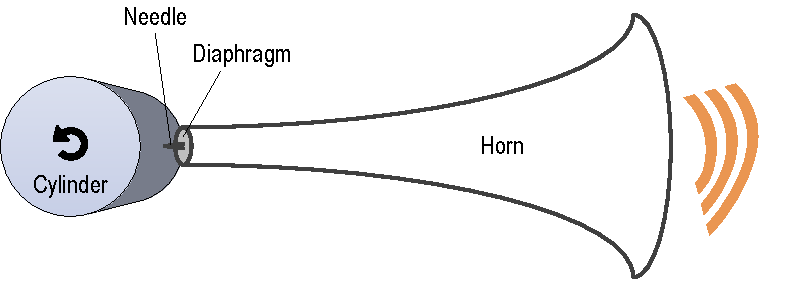
\includegraphics[width=0.9\textwidth]{images/phono-schema}
\caption{Schema of a simple phonograph.}
\label{fig:phonoschema}
\end{figure}

Then, to reproduce the recorded sound, the cylinder is repositioned at its starting position. In the original Edison phonograph, there is in fact another needle on the other side. This needle is connected to a more sensitive diaphragm so that when the crank is turned, the needle follows the previously embossed groove which causes the diaphragm to vibrate and returns the sound waves through the tube. This is then approximately the inverse process as the recording.

\subsection{Record types}
\label{sec:rectypes}

\subsubsection{Direct and stamped recordings}

The first important distinction is the way records are recorded. This also defines the different used materials. Firstly, the records made for direct recording are made to be recorded one time and play back directly with the adapted phonograph. This category is the most important for recovering nowadays because they are originally no other copies available. It includes the following record types:

\begin{itemize}
\item Wax cylinders and discs
\item Lacquer (also called acetate discs)
\item Aluminum discs
\item Plastic belt (e.g. used by the Dictabelt recorder)
\end{itemize}

The other main category are the stamped (or molded) records. These are the recordings typically encountered on the market. The original recording is firstly molded on a master, and a lot of different copies can be created by stamping on other discs. The typical examples are the following:

\begin{itemize}
\item Shellac records
\item Vinyl records
\end{itemize}

\subsubsection{Groove modulation}

The Edison phonograph uses a groove that undulates vertically. However, a lot of records, particularly the discs, have later used laterally modulated grooves. This way, it is no more the depth that determines the signal, but rather the lateral position of the groove bottom. The difference can be clearly seen in \autoref{fig:groovesdiff}.

\begin{figure}[!ht]
    \begin{subfigure}[b]{0.49\textwidth}
    \centering
    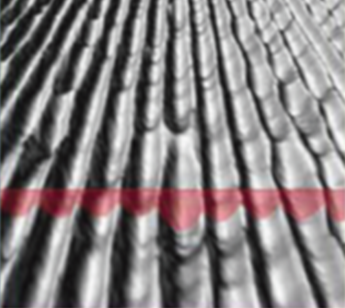
\includegraphics[width=0.8\textwidth]{images/grooves-vertical}
    \caption{Vertically modulated.}
    \label{fig:groovesvert}
    \end{subfigure}
    \begin{subfigure}[b]{0.49\textwidth}
    \centering
    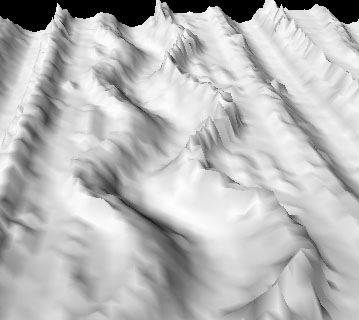
\includegraphics[width=0.8\textwidth]{images/grooves-lateral}
    \caption{Laterally modulated.}
    \label{fig:grooveslat}
    \end{subfigure}
    \caption{The two types of groove modulation.}
    \label{fig:groovesdiff}
\end{figure}

It exhibits a 3D representation of record surfaces for both groove types. In \autoref{fig:groovesvert} the boundaries are straight and the depth varies while in \autoref{fig:grooveslat} they form an horizontal wave.

\subsubsection{Revolution per minute}

Another important parameter is the number of revolutions per minute, abbreviated \emph{rpm}. It represents the rotational speed of the record while recording or playing. The speed of early records was not standardized, and it could vary from \SIrange[range-units=single]{60}{160}{rpm} for cylinders. Then, the speed has been progressively standardized to the common \SI{78}{rpm}. A lot of recording material to be restored now uses this format. The newer vinyl discs have then used the well-known speeds of \SI[quotient-mode = fraction,fraction-function = \tsfrac,output-product=\hspace{0.5pt},product-units = single]{33x1/3}{rpm} and \SI{45}{rpm}.

\section{Summary}

This chapter gave an idea of the phonograph history and different devices, showing the heterogeneous nature of the audio recording, with a lot of different techniques and materials. This outlines the difficulties that might appear while trying to recover old recordings.

The next chapter will discuss the technology developed at \gls{lbnl} in order to extract optically the sound from old records.

\chapter{Acquisition and processing systems}
\label{chap:acqprocsys}

This chapter details the systems used in the audio laboratory at \gls{lbnl} to extract records. For both systems, the main process is separated in two main steps: the acquisition and the processing. The first section is an overview of the setup and hardware used to acquire records, followed by the characteristics of this acquisition step. The last two sections present the specificities of each system, both about acquisition and processing steps.

\section{Acquisition hardware}

Both \gls{irene} and \gls{3dprobe} use the same hardware for the acquisition. It consists of different sensors and motors connected to a controller. This controller is itself driven by a software, using a special library embedded in a \gls{labview} environment.

\subsection{Components}

There are two main different supports. The first one is a turntable specifically designed for flat discs with the scanner put vertically and the disc rotating horizontally. The second one enables cylinder scanning, the probe being placed horizontally and directly facing the record. \autoref{fig:labhw} represent the installation in the laboratory.

\begin{figure}[!ht]
    \begin{subfigure}[b]{0.49\textwidth}
    \centering
    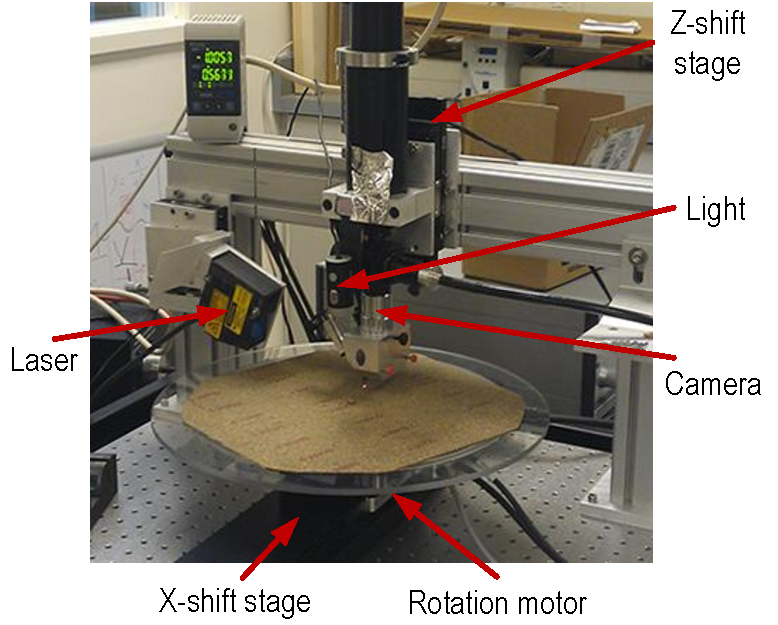
\includegraphics[width=\textwidth]{images/hardware-irene}
    \caption{The turntable to acquire flat discs.}
    \label{fig:labirene}
    \end{subfigure}
    \begin{subfigure}[b]{0.49\textwidth}
    \centering
    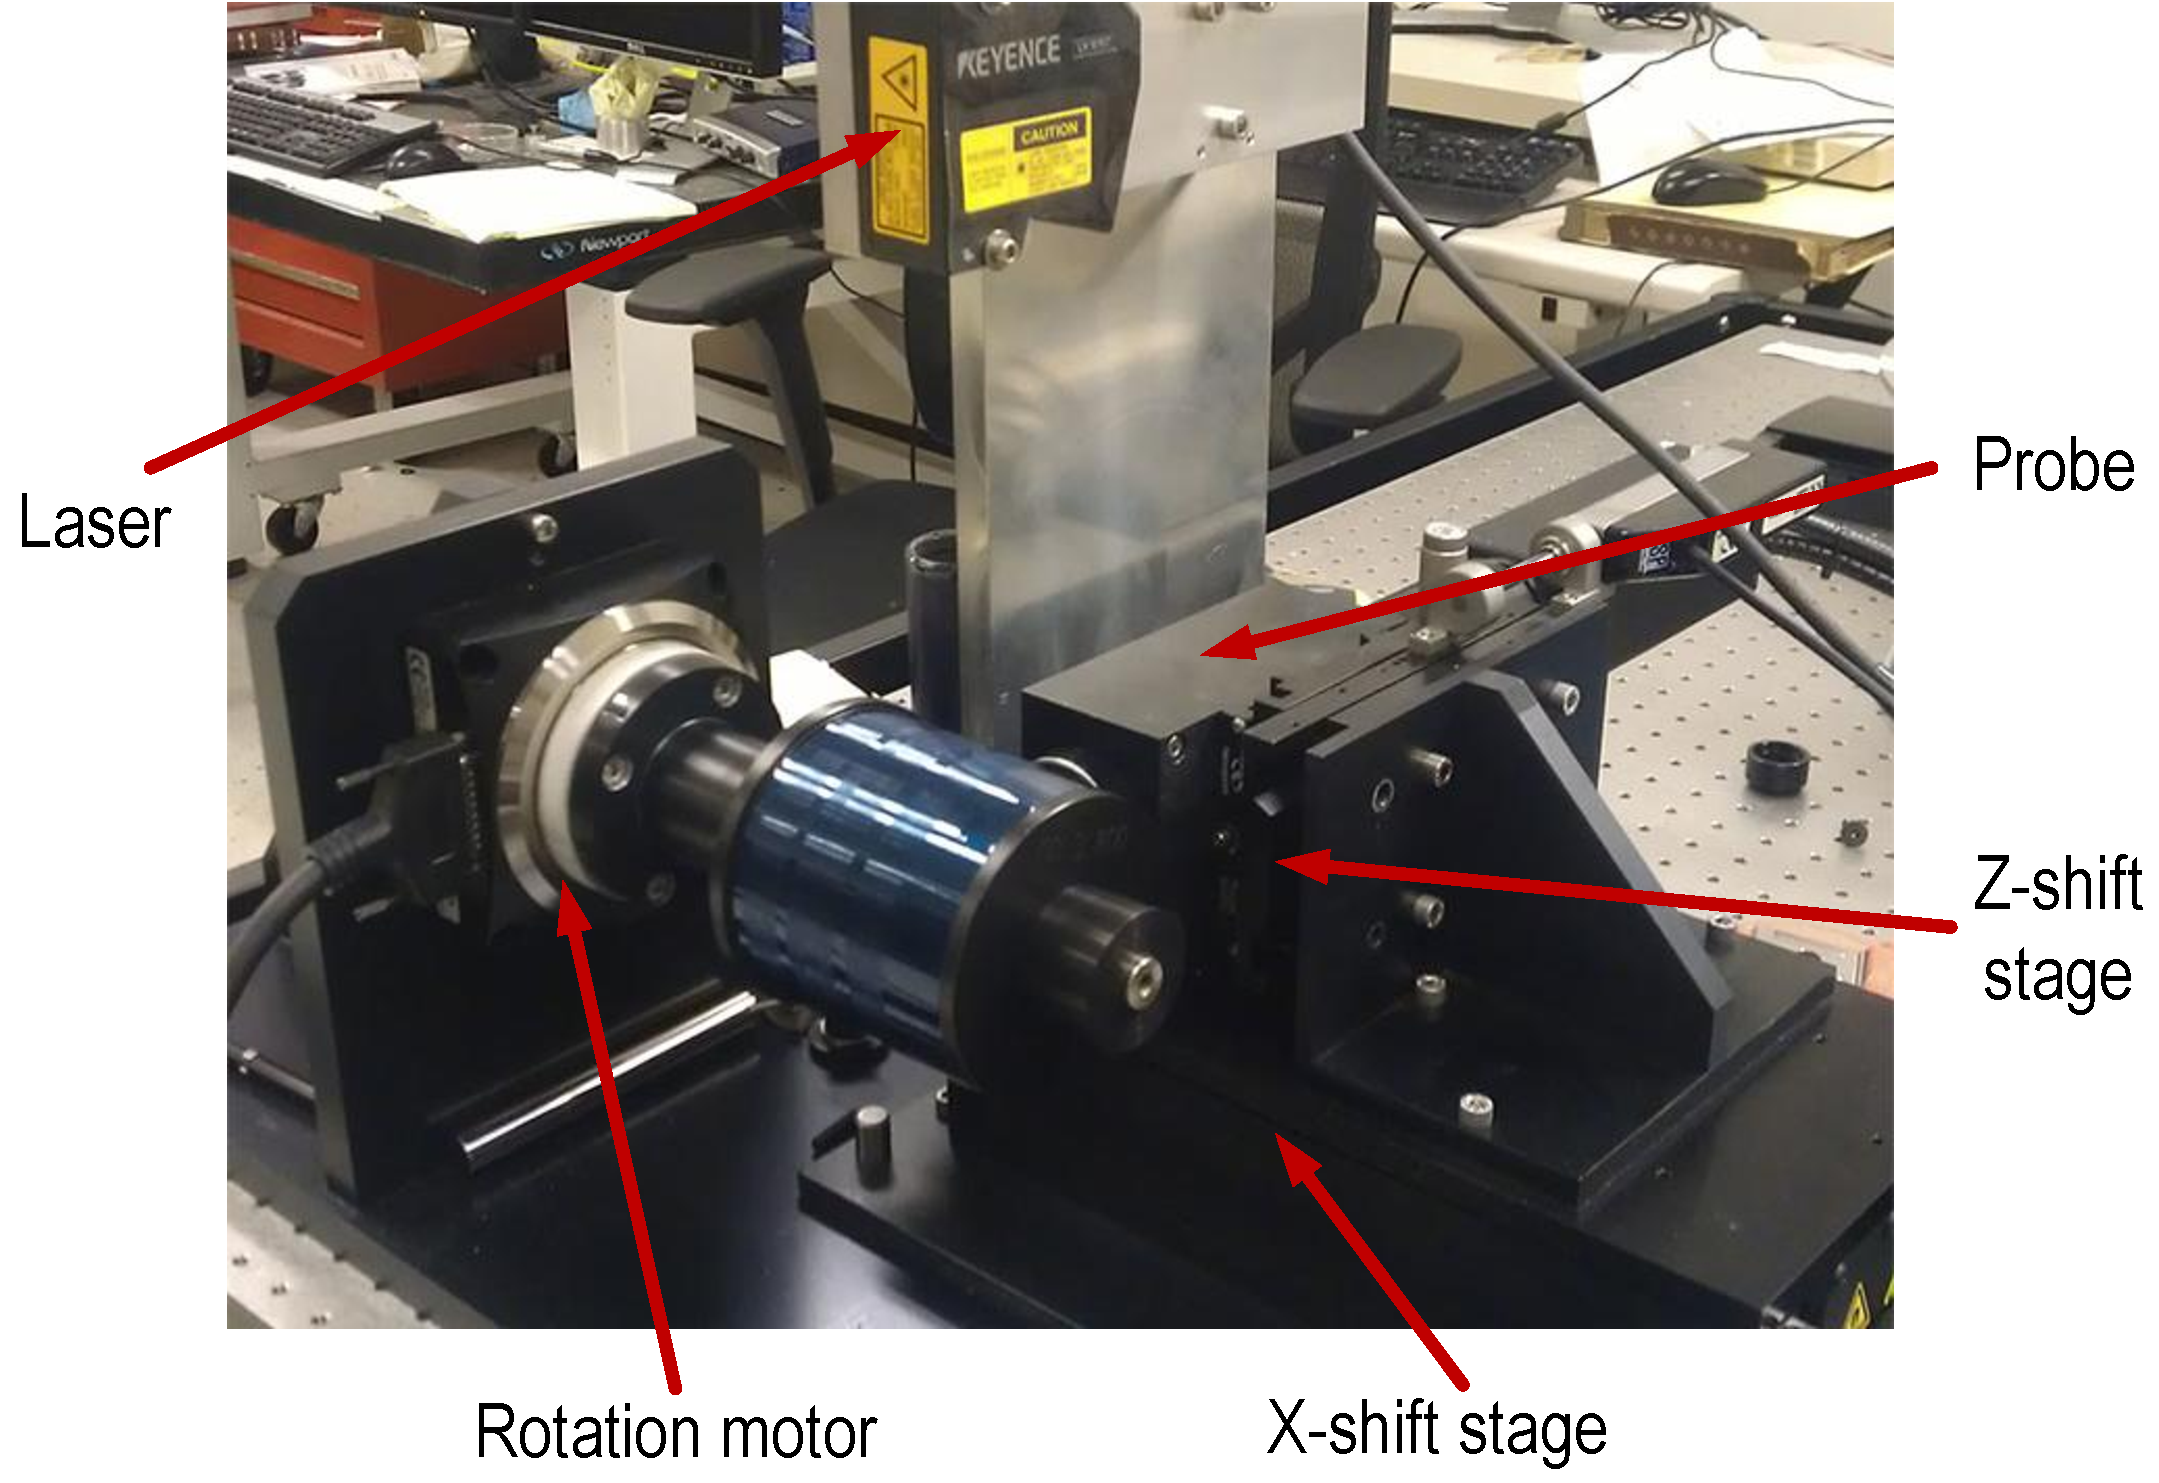
\includegraphics[width=\textwidth]{images/hardware-3d}
    \caption{The scanning equipment for cylinders.}
    \label{fig:lab3d}
    \end{subfigure}
    \caption{The acquisition hardware as installed at LBNL.}
    \label{fig:labhw}
\end{figure}

In both cases, in addition to the rotary motor, there is a X- and Z- shifting motor. The X-motor enables to shift the record to scan another portion. The Z-motor is used to adapt the sensor height for a correct focus.

\subsection{Z-correction}
\label{sec:zcorr}

Small differences can cause the 2D image to be blurred or the 3D scan to be out of range. To avoid this problem, a Z-shift correction is applied. The height shifting is controlled using a laser displacement sensor. It follows up the record and adjusts the sensor height, acting as an ``autofocus system''.

\section{Mapping characteristics}
\label{sec:mapping}

Before explaining the specificities of each system, it is noteworthy to explain the basic concepts about record acquisition used in both 2D and 3D systems. The most important is to understand the mapping of a record onto a 2D image. This characteristic is slightly different from the two categories, cylinders or discs.

\subsection{Disc mapping}

As previously seen in \autoref{fig:labirene}, the setup for flat discs acquisition looks similar to an ordinary phonograph. The disc is placed on the turntable and rotates while the sensor takes a single line of capture at regular intervals.

The first main difference is that an entire revolution may acquire more than a single groove (as it would be played by a phonograph needle). The line width and other properties depend on the sensor and will be detailed in the next sections.

Since each captured line are put together, an entire revolution finally results in a ring-shaped capture which is mapped in a rectangular image. The groove then maps to straight parallel lines instead of the original spiral. This mapping is more clearly seen in \autoref{fig:discmapping}.

\begin{figure}[!ht]
    \begin{subfigure}[t]{0.48\textwidth}
    \centering
    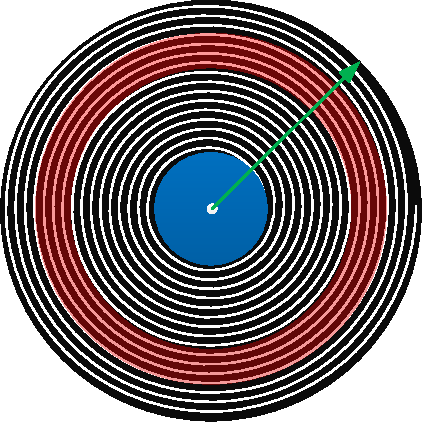
\includegraphics[width=0.9\textwidth]{images/mapping-disc-orig}
    \caption{Portion of the captured ring.}
    \label{fig:discmappingorig}
    \end{subfigure}
    \begin{subfigure}[t]{0.48\textwidth}
    \centering
    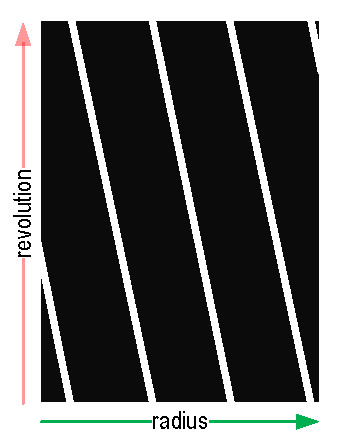
\includegraphics[width=0.75\textwidth]{images/mapping-disc-img}
    \caption{Mapping as a rectangular image in polar coordinates (scaled).}
    \label{fig:discmappingimage}
    \end{subfigure}
    \caption[Schema representing mapping of a flat disc.]
    {Schema representing mapping of a flat disc. The example groove is enlarged a lot from reality for a proper visualization. The right image corresponds to the red portion on the disc.}
    \label{fig:discmapping}
\end{figure}

It is important to note that as the mapping represents a revolution, the resulting \emph{top} and \emph{bottom} of the acquisition are in fact at the same position. As the groove is embossed as a spiral onto the disc surface, the result is not exactly vertical but slightly inclined. The groove section ending at the image bottom continues at the same horizontal position at the top (or vice versa depending on the capture direction). A radial line maps to a line (almost) perpendicular to the grooves

\subsubsection{Off-axis problem}

This section explained the general idea of mapping. However, in practical situations, the groove shape is rarely so straight on the mapped image. Instead, it results in waved repeated sections, as seen in \autoref{fig:offaxise}.

\begin{figure}[!ht]
\centering
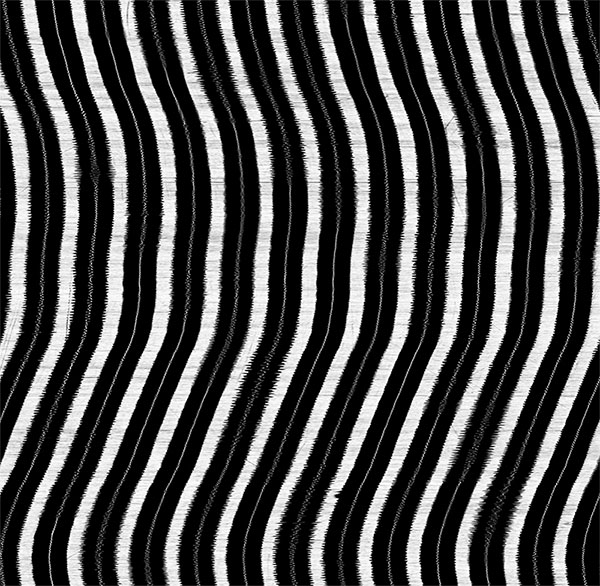
\includegraphics[width=0.5\textwidth]{images/off-axis}
\caption{Example of a mapped entire revolution acquisition with off-axis.}
\label{fig:offaxise}
\end{figure}

This result comes from the fact that the disc is hardly \emph{exactly} put at the center of the turn table. As a groove is in reality very tight, a small off-axis of e.g. \SI{0.5}{\milli\metre} is already clearly visible on a capture of a whole revolution.

However, the distortion is only problematic for visualization. The resulting sound is not altered, even for laterally-modulated records, as the frequency is very low compared to the actual embossed signal.

\subsection{Cylinder mapping}

Because of the geometrical shape, the cylinder mapping is slightly different. Again, the cylinder rotates in a way similar to the original Edison phonograph, while the sensor captures lines. A whole revolution gives an image equivalent to the disc mapping, as seen in \autoref{fig:cylmapping}.

\begin{figure}[!ht]
    \begin{subfigure}[t]{0.45\textwidth}
    \centering
    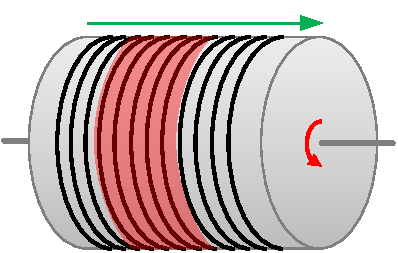
\includegraphics[width=\textwidth]{images/mapping-cyl-orig}
    \caption{Portion of the captured strip.}
    \label{fig:cylmappingorig}
    \end{subfigure}
    \begin{subfigure}[t]{0.45\textwidth}
    \centering
    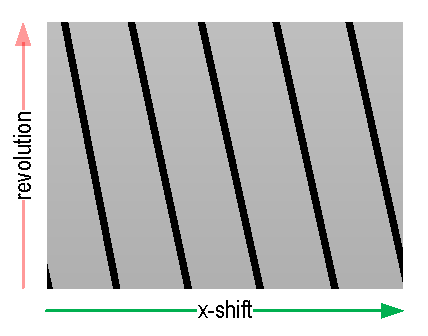
\includegraphics[width=0.8\textwidth]{images/mapping-cyl-img}
    \caption{Mapping as a rectangular image in polar coordinates (scaled).}
    \label{fig:cylcmappingimage}
    \end{subfigure}
    \caption[Schema representing mapping of a cylinder.]
    {Schema representing mapping of a cylinder. The example groove is enlarged a lot from reality for a proper visualization. The right image corresponds to the red portion on the record.}
    \label{fig:cylmapping}
\end{figure}

This time, the mapped representation corresponds to an unrolled cylinder strip. Another way of viewing this if as if we unwrap the tinfoil around an Edison cylinder and look at it unfolded. This time, a line perpendicular to the grooves maps also to a perpendicular line on acquired image, and a vertical lines remains vertical. The Y coordinates corresponds to the rotation angle.

\section{Binned representation}
\label{sec:binrepr}

A record complete acquisition gives an image in very high resolution, so that the sample rate is big enough \footnote{The complete discussion about sample rate is given in the corresponding next sections for \gls{irene} and \gls{3dprobe}.}. It is often useful to have a more general view of the record. Particularly, to view an entire revolution, all points in the vertical axis are not useful. Both systems create then a \emph{binned} image, which corresponds to the acquired image with the height divided by a certain factor $d$, typically around \numrange[range-phrase=--]{20}{100} that can be changed according to the original resolution. It is created by averaging the value of the actual pixel values every $d$ lines. The result is an image such as the one already viewed in \autoref{fig:offaxise}.

In addition to the visualization, this representation will be very useful for a step of the processing algorithm, which will be explained in the next sections.

\section{IRENE}

\subsection{Acquisition}

As already explained, \gls{irene} uses numerical 2D capture for the acquisition. The scanner takes some monochromatic pictures of the disc. The resulting image is influenced by the shape of the surface because of the light reflection. This enables to visually find the grooves on the resulting picture. An example of such a picture is shown in \autoref{fig:irenecapex}.

\begin{figure}[!ht]
\centering
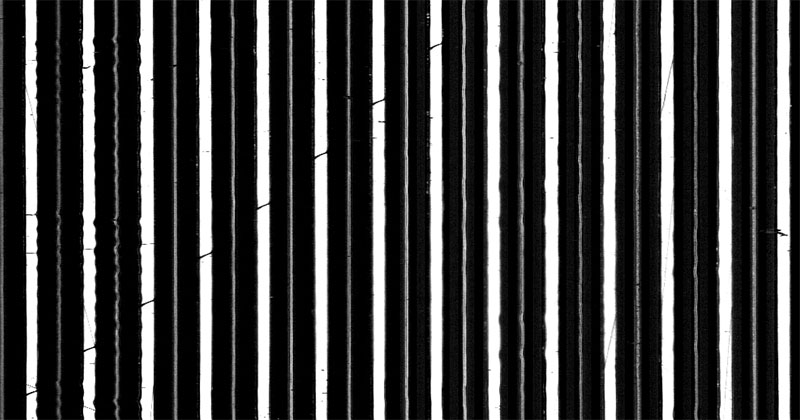
\includegraphics[width=0.7\textwidth]{images/irene-capture-ex}
\caption{IRENE capture excerpt.}
\label{fig:irenecapex}
\end{figure}

A single groove can be seen as two black strips with a thin bright line in between. The black parts represent the edges while the thin line is the bottom of the groove. Between two grooves, the interval also appears in white. \autoref{fig:irenegroove} describes the different parts.

\begin{figure}[!ht]
\centering
    \begin{subfigure}[t]{0.29\textwidth}
    \centering
    \raisebox{0.3cm}{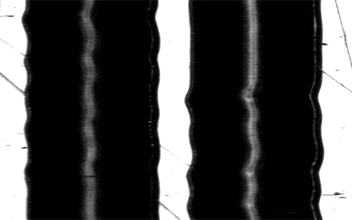
\includegraphics[width=4cm]{images/irene-grooves}}
    \caption{Two scanned grooves.}
    \label{fig:irenegrimg}
    \end{subfigure}
    \begin{subfigure}[t]{0.7\textwidth}
    \centering
    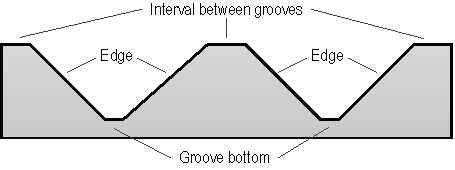
\includegraphics[width=9.5cm]{images/irene-grooves-schema}
    \caption{The corresponding shape.}
    \label{fig:irenegrschema}
    \end{subfigure}
    \caption{Visualization of scanned grooves.}
    \label{fig:irenegroove}
\end{figure}

\autoref{fig:irenegrimg} represents two grooves as they appear from the acquisition part. The approximate corresponding shape in a sectional view is visualized in \autoref{fig:irenegrschema}.

\subsubsection{Coaxial illumination}

The system uses coaxial illumination. Every light beam is parallel and orthogonal to the record surface. Therefore, the intensity of the resulting pixels will finally depend on the slope of the surface, as visualized in \autoref{fig:irenecoaxlum}.

\begin{figure}[!ht]
\centering
    \begin{subfigure}[t]{0.48\textwidth}
    \centering
    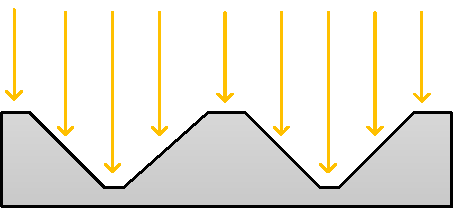
\includegraphics[width=0.9\textwidth]{images/irene-lum-emi}
    \caption{Light emission.}
    \label{fig:irenlumemi}
    \end{subfigure}
    \begin{subfigure}[t]{0.48\textwidth}
    \centering
    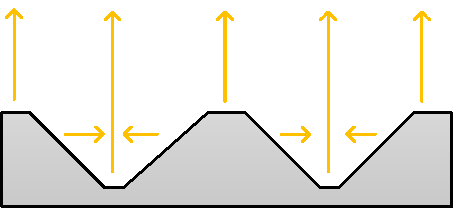
\includegraphics[width=0.9\textwidth]{images/irene-lum-reflect}
    \caption{Light reflection.}
    \label{fig:irenelumreflect}
    \end{subfigure}
    \caption[Coaxial illumination, light emission and reflection.]
    {Coaxial illumination, light emission and reflection. The light is not reflected back to the source on groove edge, resulting in black parts on the acquired image.}
    \label{fig:irenecoaxlum}
\end{figure}

On the exact groove bottom, the slope is null and then the light is orthogonally reflected. This is also valid for the interval between two grooves, as the surface is almost flat. On the other hand, the groove edges are very sloping and the light is not reflected directly to the source. The corresponding pixels will then appear black.

\subsubsection{Capture properties}

The camera cannot take a whole picture of one disc in a snapshot. It captures a line of \SI{3.072}{\milli\metre} with \num{4096} pixel samples. For a total disc revolution, \num{80000} lines are captured this way. Therefore, it results in an image of \SI[product-units=single]{4096x80000}{px} representing a ring-shaped disc capture in polar coordinates. To simplify the manipulation, the high resolution image is exported as eight separate pictures of \SI[product-units=single]{4096x10000}{px} easier to process.

For a \SI{78}{rpm} disc, the time for one revolution $t_{cyc}$ is the inverse of the rotational speed $w_{cyc}$. Therefore, the sampling rate $f_s$ for the system is given by

\begin{equation}
\label{eq:samprateirene}
f_s = \frac{n_{sample}}{t_{cyc}} = \frac{n_{sample}}{\frac{1}{\omega_{cyc}}} = \frac{\num{80000}}{\frac{1}{\SI{78}{rpm} \cdot \SI[quotient-mode=fraction]{1/60}{\metre\per\second}}} \approx \SI{104}{\kilo\hertz}
\end{equation}

This value satisfies the sampling theorem\footnote{The Nyquist–Shannon sampling theorem states that the minimum sampling frequency should be greater than twice the maximum of the sampled signal to reconstruct it properly. As the human hearing have a range from \SIrange[range-units=single]{20}{20000}{\hertz}, the sample rate for audio signal must be at least \SI{40}{\kilo\hertz}.} as it is greater than the minimum of \SI{40}{\kilo\hertz}.

\subsection{Processing}
\label{sec:reneprocessing}

During the acquisition, the original record is digitized and can be archived on digital media. To extract the sound, the next step is to use the \gls{rene} program. It offers features to process the record images and output the final corresponding sound as a \gls{wav} file.

\gls{rene} embeds a lot of algorithms and parameters to adapt at best the processing to the different record types. It is written in the \Csh{} programming language, enabling to easily build a complete graphical application without the use of third-party libraries. The \gls{gui} simplifies its utilization and offers the possibility to visually follow the tracking, as seen in \autoref{fig:irenegui}.

\begin{figure}[!ht]
\centering
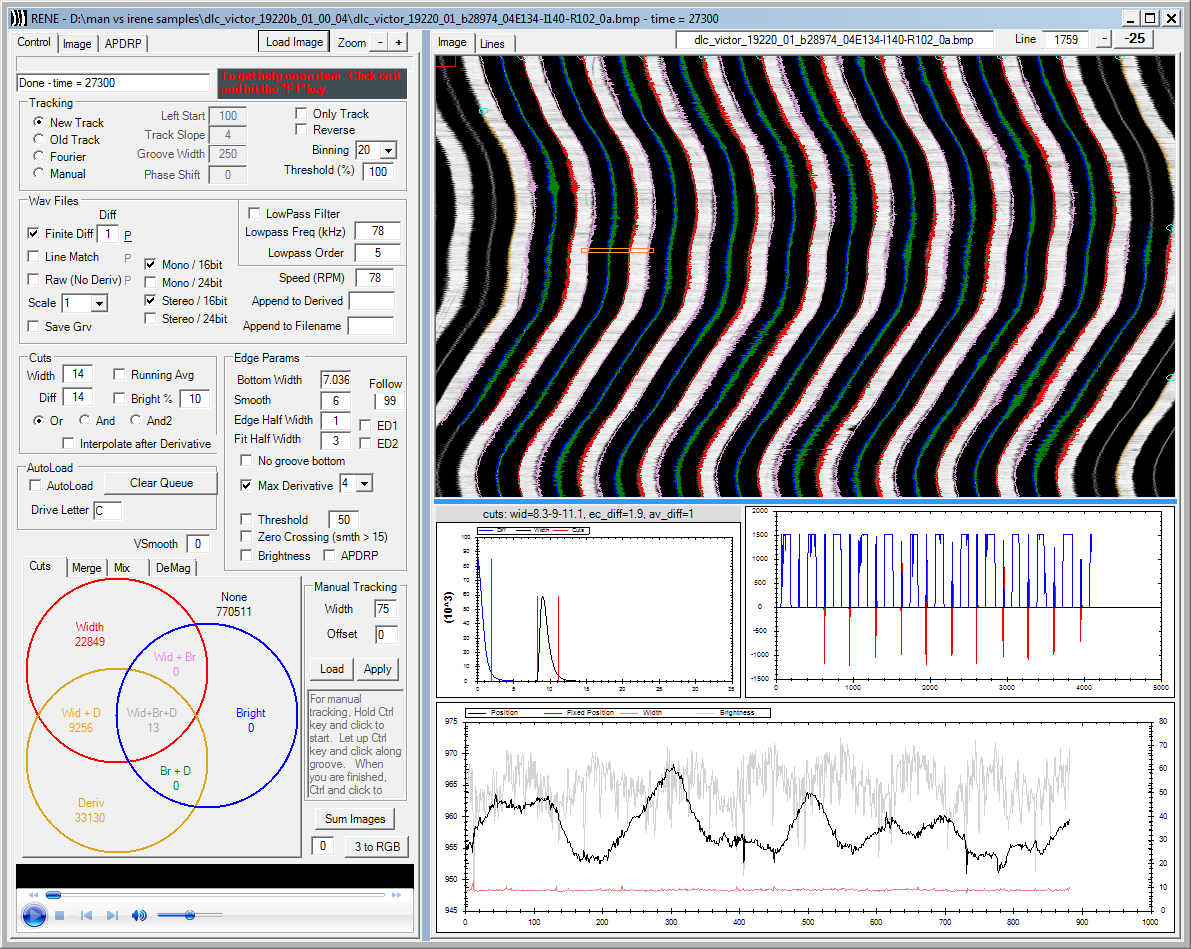
\includegraphics[width=0.9\textwidth]{images/rene-gui}
\caption{The IRENE user interface.}
\label{fig:irenegui}
\end{figure}

The left panel is used to specify the different parameters and algorithms for the separate steps and more generally to control the application. The upper right panel shows the processed record image. When the tracking is applied, the detected edges are directly drawn on top of the image. The panel at the bottom presents diverse information and statistics on the records.

The whole processing is applied in several steps.

\subsubsection{Tracking}

The tracking is the first step to process a disc. It enables to approximately find the groove positions on a record using different detection algorithms. These latter are performed on the binned image (see \autoref{sec:binrepr}). It is actually the one seen in the upper right panel in the \gls{gui} (see \autoref{fig:irenegui}).

Due to the small bitmap size, this processing is consequently very efficient and not subject to possible noise or imperfections which are smoothed by the binning. In the user interface, the result of this step can be viewed on the top-panel as the purple and red external lines delimiting the grooves as seen in \autoref{fig:irenegui}.

Several different algorithms (explained in detail in \autoref{sec:trackmethods}) can be selected to track the grooves. The best one to apply depends on the scanned medium and its general condition. As already mentioned, there is also an option to manually define the groove position when automatic methods are not applicable (e.g. if the disc is too damaged). The user can directly select points that define an interpolated line, which must follow the edge of the groove. This feature will be further explained in \autoref{sec:mancurrentimpl}.

\subsubsection{Image processing}

The next step is the actual processing. When the grooves are tracked, it remains to precisely find the groove center, which defines the sound information. Again, different algorithms can be used as methods using the derivative, thresholding, etc.

The result is the precise groove bottom defined between the blue and green traces on \autoref{fig:irenegui}.

\subsubsection{Sound processing}

Finally, it remains to create the output \gls{wav} file from the tracked groove bottom positions. At this step, some filters can also be applied to improve the sound quality.

\subsection{Architecture}

The diagram in \autoref{fig:renearchi} presents the general architecture of RENE.

\begin{figure}[!ht]
\centering
\includegraphics{diagrams/rene-gen-design.1}
\caption{General architecture of RENE.}
\label{fig:renearchi}
\end{figure}

The program does not use object-oriented design. The business logic and processing parts are embedded in the \texttt{Form1} class which also represents the view of the application (inheriting from the .NET WinForms \gls{api}).

Dependencies between the different classes are then fairly simple. Some tasks have been separated in external classes contained in the \texttt{Form1} class, as for the groove tracking or image processing which includes in fact routines to load images into bitmaps. The \texttt{DB} class handles connection and communication with a database, used to automatically store information and statistics on the processing results in a centralized database.

Some common processing tasks are separated in different utility classes, e.g. \gls{fft} algorithm or \gls{wav} processing to output the sound file.

\section{3D Probe}

\subsection{Acquisition}

With \gls{3dprobe}, the acquisition stage is the main difference. Instead of using a regular camera, a special probe is used, getting the actual depth for each point over a scanned part. This gives a real heightmap of the disc surface, as shown in three-dimensional view in \autoref{fig:groovesdiff}.

To measure the height of the scanned surface, the sensor takes advantage of the chromatic aberration \footnote{Optical distortion occurring when a lens cannot properly focus all colors of a same point due to different refractive indices for different wavelengths of the light.}. Light is emitted and passes through an objective. Because the refraction index depends on the wavelength, the light is refracted differently regarding the wavelength, as shown in \autoref{fig:chromaber}.

\begin{figure}[!ht]
\centering
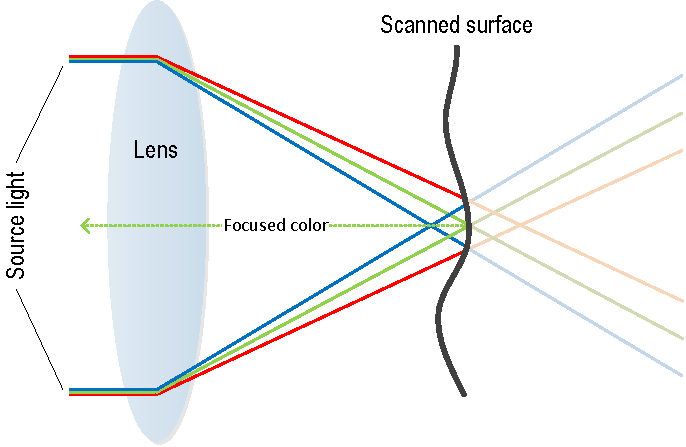
\includegraphics[width=0.8\textwidth]{images/chromatic-aberration}
\caption{Chromatic aberration through a lens.}
\label{fig:chromaber}
\end{figure}

Hence, the color reflecting in focus on the surface will depend on the distance from the lens. The sensor captures then the reflected wavelength and can deduce the height. The probe can also give the value of the brightness, that is, the captured light intensity for a given point.

\subsubsection{Capture properties}
\label{sec:3dcaptureprop}

In a single snapshot, the sensor is able to capture 180 points in one line of \SI{1.8}{\milli\metre} in a way similar to the 2D camera with \gls{irene}. The depth is measured in a range of \SI{400}{\micro\metre} with a resolution of \SI{0.125}{\micro\metre}.

The acquisition software outputs the data in a specific binary file format with extension \emph{.pri}, containing essentially floating-point values corresponding to the depth captures. The brightness is stored separately in a \emph{.bri} file, using exactly the same structure.

In this case, the number of samples for a full revolution depends on the angle $\alpha$ by witch the cylinder is rotated between two samples. Therefore, the sampling rate is not fixed and the formula for a cylinder at \SI{160}{rpm} become
%
\begin{equation}
\label{eq:samprate3d}
f_s = \frac{n_{sample}}{t_{cyc}} = \frac{n_{sample}}{\frac{1}{\omega_{cyc}}} = \frac{\frac{\ang{360}}{\alpha}}{\frac{1}{\SI{160}{rpm} \cdot \SI[quotient-mode=fraction]{1/60}{\metre\per\second}}}
\end{equation}
%

For example, with an angle $\alpha$ of \ang{0.02}, the number of samples is $\frac{\ang{360}}{\ang{0.02}} = \num{18000}$ and the sampling rate become $\frac{\num{18000} \cdot 160}{60} = \SI{48}{\kilo\hertz}$.

\subsubsection{Multiple-pass acquisition}

From the capture properties, the distance between two points is \SI{10}{\micro\metre}. The corresponding resolution is then quite low and could not be enough in some cases.

Therefore, the \gls{labview} acquisition software is able to perform a multiple-pass scanning. The same part a record is captured several times with a different shift. For example, by using two-pass, the number of points, and so the resolution are multiplied by two resulting in 360 points for the same distance.

\subsection{Processing}

The processing is done with the program called \gls{prism}. It uses the data stored in the \emph{.pri} and \emph{.bri} files to process and output the sound. The application is very similar to \gls{rene} and is also written in \Csh. There are also a lot of different parameters to tune the tracking and processing at best for the corresponding record type. Some parameters are also specifically related to cylinder processing.

The user interface (\autoref{fig:prismgui}) embeds approximately the same main parts as \gls{rene}, though differently disposed.

\begin{figure}[!ht]
\centering
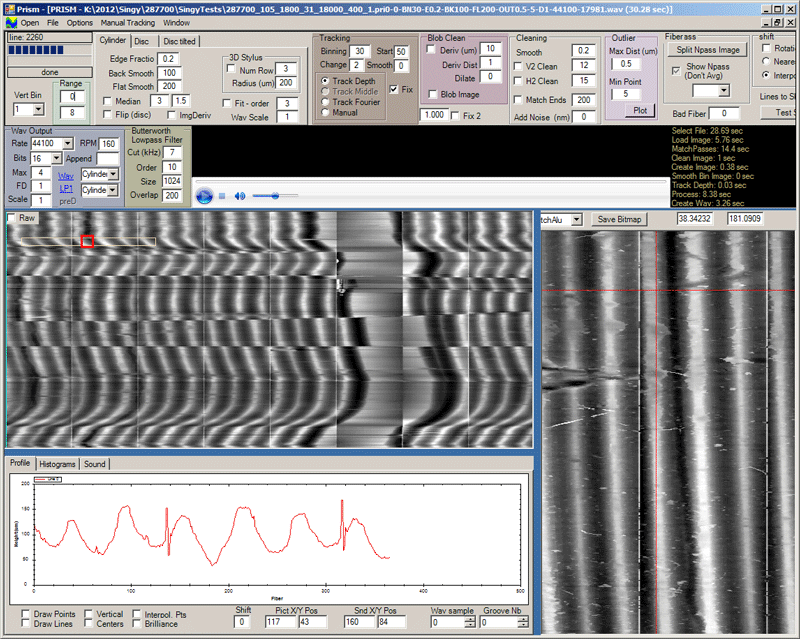
\includegraphics[width=0.9\textwidth]{images/prism-gui}
\caption{The PRISM user interface.}
\label{fig:prismgui}
\end{figure}

The parameters and algorithms can be set on the top panel. In the middle and the right, the scanned media is visualized as a 2D heightmap. The dark and bright colors emphasize the higher, respectively the lower points on the surface. The image at the left-hand side is a general view while the other one shows a full resolution portion of the record (selected with the cursor and highlighted with the red square on the left panel). The lower panel gives the same type of information as the other program.

\subsubsection{Processing steps}
\label{sec:3dprocsteps}

The processing part is performed through the same steps as with \gls{rene} (see~\autoref{sec:reneprocessing}). The main point is to take into account that a pixel value now denotes a real height and no more a brightness difference as on a photography. Likewise, the 3D acquisition suffers from bad points, that is, pixels with incorrect height value coming from the acquisition. Special algorithms are then set up to clean the scanned data and suppress these bad points.

Finally, the cylinder processing algorithm is specific, as it considers of course the vertically engraved nature of these type of record (see~\autoref{sec:rectypes}). The waveform is indeed defined by the surface height in the groove bottom (the intensity in the heightmap) and not by its lateral position.

\subsection{Architecture}
\label{sec:prismarchi}

The general architecture of \gls{prism} is presented in \autoref{fig:prismarchi}.

\begin{figure}[!ht]
\centering
\includegraphics{diagrams/prism-gen-design.1}
\caption{General architecture of PRISM.}
\label{fig:prismarchi}
\end{figure}

The \gls{prism} program have a refined architecture, using more object-oriented facilities. The \gls{gui} is handled by the \texttt{frmMain} class. The big part of the business logic has been separated in its own class \texttt{Hardware}. This class represents an abstract record which is processed by the application. A inheritance hierarchy is built from it, mainly separated in \texttt{Cylinder} and \texttt{Disc} types representing vertically and laterally engraved records. This design enables to specialize the algorithms for any types of records.

Other utility classes handle common processing such as \gls{wav} creation or signal cleaning algorithms.

\section{Typical records issues}

As already stated, a lot of important and historical recordings are still stored on old records without other copies. Many of them can no more be read with regular phonographs. \gls{irene} and \gls{3dprobe} systems can then be used to restore the sound. However, some of the recordings are already altered, e.g. with some cracks appearing on disc surface, or completely broken into pieces, as old cylinders. These latter can still be acquired in several steps by strapping the pieces together, resulting in the same kind of issues in the processing step.

Depending on the degradation level, other issues can also appear with optical methods. In some cases the systems are still not able to perform a proper scan. The next sections depict the most common problems.

\subsection{Shifting}
\label{sec:issueshift}

Visible cracks on a record as shown in \autoref{fig:crackeddisc} is only the tip of the iceberg. Usually, it involves other problems to be solved algorithmically. One of the most common problem is shifting. When different parts of a disc surface are separated because of the cracks, they typically move slightly from each other, resulting in grooves mismatch. An example of this kind of issue is illustrated in \autoref{fig:shiftedgrooves}.

\begin{figure}[!ht]
\centering
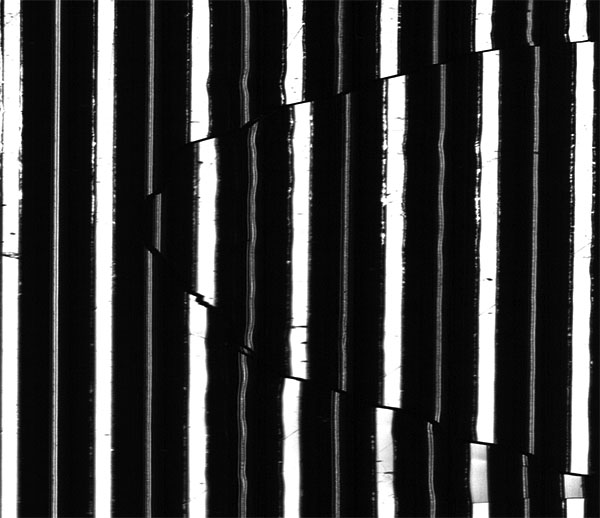
\includegraphics[width=0.6\textwidth]{images/shifted-grooves}
\caption{Grooves shifted because of a crack.}
\label{fig:shiftedgrooves}
\end{figure}

The acquisition shows clearly the two distinct pieces separated by a arch-shaped crack. In this case, the grooves are only slightly shifted. However the difference can be much larger and exceed up to several grooves large, causing difficulty to visually find the correct matching.

\subsection{Focus}

As explained in \autoref{sec:zcorr}, the acquisition needs always to stay in focus to get a sharp image. However, when the height varies abruptly, the laser is not able to directly compensate the Z-shift. This can happen sometimes when the lacquer inflates resulting in bubbles on the surface. The result in the acquisition is shown in \autoref{fig:blurredgrooves}.

\begin{figure}[!ht]
\centering
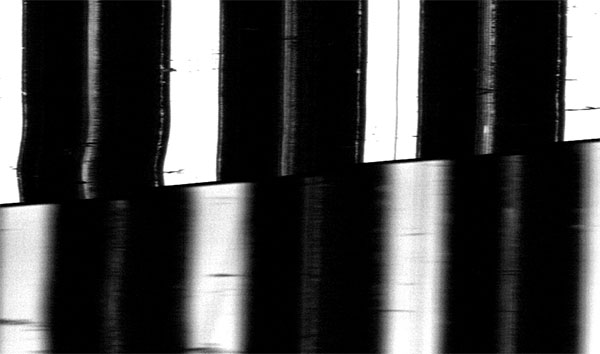
\includegraphics[width=0.6\textwidth]{images/blurred-grooves}
\caption{Blurred grooves on the bottom part under the crack.}
\label{fig:blurredgrooves}
\end{figure}

\subsection{Other issues}

Other problems may occur because of the cracks. For example, because of the lacquer deformation, the pieces can sometimes expand or shrink, which results in other corrections to apply. Likewise, the gaps introduced by the cracks can sometimes be large and the resulting sound affected. Most of time, the gap is not a loss of content but rather a separation due to the shrinkage. Yet the reciprocal can also happen, i.e. when a piece of lacquer coat is folded on another one.

The trouble is to find out what is the best interpolation scheme to match the sound between the cracks. Furthermore, these latter issues become more important when a sound has to be synced with a visual representation, as for a movie sound track for example. The sound must match the picture so that the film is properly watchable.

\section{Sample recordings}
\label{sec:samplerec}

To investigate properly on the previously discussed issues, a canonical test set has been provided by the laboratory. These samples gather the typical problems that the current software components are unable to process correctly. Their properties as well as a general analysis of the related issues will be detailed in the next sections.

\subsection{Graham Bell disc}

A collection of Graham Bell records\footnote{More information on the recovered collection can be found on this IRENE web page: \url{http://bio16p.lbl.gov/volta-release.html}.} has been recovered using the IRENE \gls{3dprobe} at the Library of Congress in Washington DC. This collection comes from the Volta Laboratory created by Alexander Graham Bell. One of the disc in the collection, labeled 287700, is a vertically-cut wax disc. It can be viewed in \autoref{fig:belldisc}.

\begin{figure}[!ht]
\centering
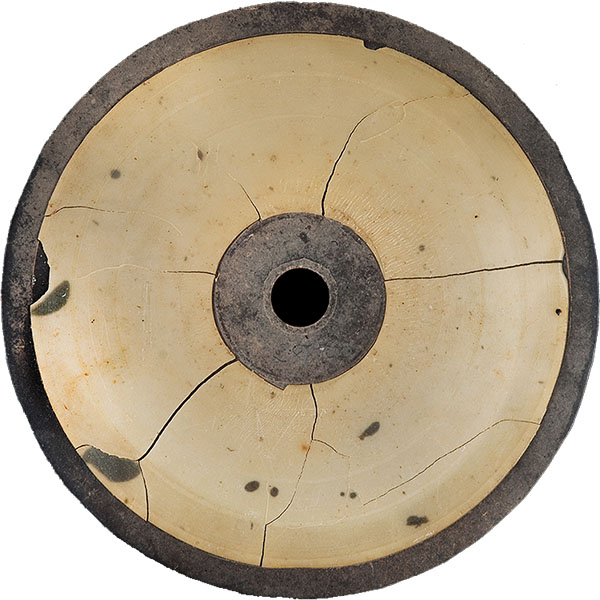
\includegraphics[width=0.5\textwidth]{images/bell-disc}
\caption[The Graham Bell 287700 disc.]{The Graham Bell 287700 disc. The radial cracks are clearly visible on the photography.}
\label{fig:belldisc}
\end{figure}

This record is cracked and the specific cracks are clearly visible as black traces on the support, revealing the material underneath the wax layer visible in a yellowish color. This disc has been acquired with the \gls{3dprobe} system, but the program is not able to properly process it. Indeed, one can clearly see that groove shifting can appear when a crack is reached, as in \autoref{fig:bellcrack}, making it impossible to track.

\begin{figure}[!ht]
\centering
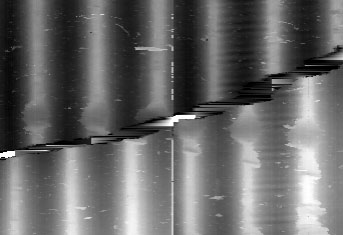
\includegraphics[width=0.7\textwidth]{images/bell-crack}
\caption{A crack on the 287700 disc as it appears in PRISM (detail image).}
\label{fig:bellcrack}
\end{figure}

On the whole record, the shifting does not seem to be very large. There is no more than one groove width of shifting in this case.

\subsection{Dickson cylinder}

This specific wax cylinder comes from an experimental project by William Dickson and Thomas Edison. It is the soundtrack recording for the first film with recorded sound in addition to the motion picture. It is then an early prototype of a sound-film, but without real synchronization between picture and sound. This first attempt of a sound-film is known as the \emph{Dickson Experimental Sound Film}.

This cylinder is seriously damaged and contains, in addition to cracks, big areas where the grooves are removed, probably due to a piece of layer that has been entirely broken. This problem can be visualized in \autoref{fig:dicksonbig}. A smaller example of a crack is presented in \autoref{fig:dicksoncrack} as it is viewed from \gls{prism} in full resolution.

\begin{figure}[!ht]
\centering
    \begin{subfigure}[t]{0.49\textwidth}
    \centering
    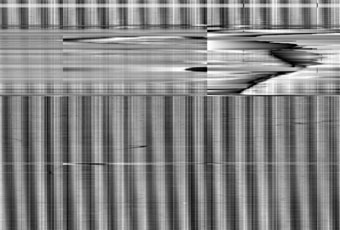
\includegraphics[width=0.9\textwidth]{images/dickson-damage-big}
    \caption{A damaged area as seen in binned view.}
    \label{fig:dicksonbig}
    \end{subfigure}
    \begin{subfigure}[t]{0.49\textwidth}
    \centering
    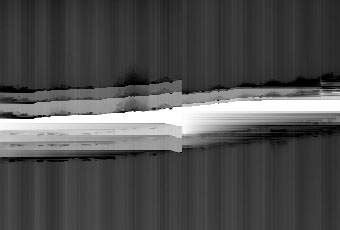
\includegraphics[width=0.9\textwidth]{images/dickson-crack}
    \caption{A small crack in detailed view.}
    \label{fig:dicksoncrack}
    \end{subfigure}
    \caption[Damages on the Dickson cylinder.]{Damages on the Dickson cylinder. In both images, the vertical grooves are hardly noticeable because when an irregularity occurs the depth difference is much bigger than the usual groove height (this is only a visualization issue).}
    \label{fig:dicksondamage}
\end{figure}

However, even with these missing parts, the shifting remains once more quite small, and the right path is quite easy to spot for a human.

\subsection{Boas recording}

Franz Boas was a famous anthropologist born in 1858 in Germany. He moved to the United States in 1887 where he started to study Native North American populations. During his researches and expeditions on Vancouver Island in 1930, Boas recorded sound. Some of these records have been acquired with \gls{3dprobe} for restoration some time ago. One of the disc in the collection, labeled 0724, is a damaged wax cylinder.

As with every cylinder, it was acquired with the \gls{3dprobe} system. This record suffers from a lot of cracks separating the data in several pieces. These separated pieces can then be quite small. \autoref{fig:0724cracks} represents a portion of the disc after the acquisition.

\begin{figure}[!ht]
\centering
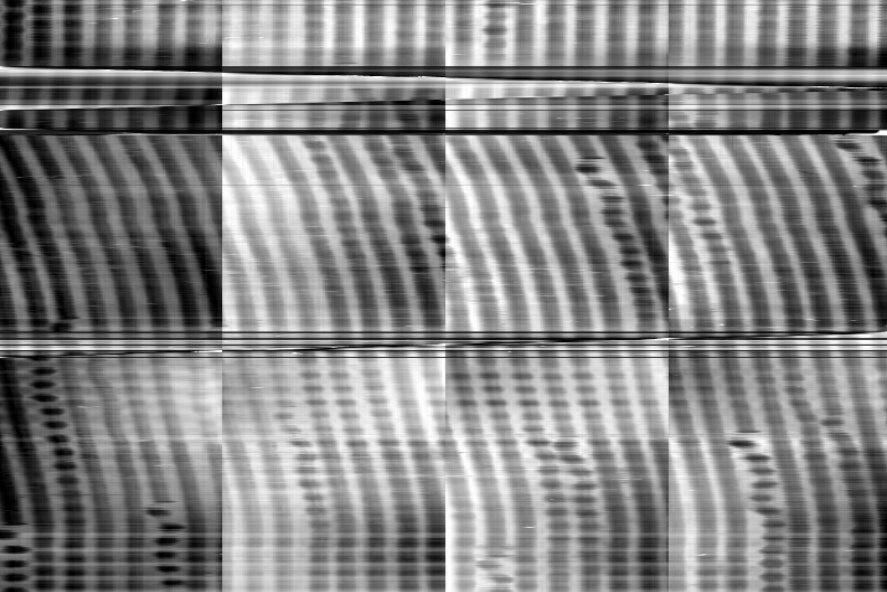
\includegraphics[width=0.7\textwidth]{images/0724-cracks}
\caption{Excerpt of the acquisition of the 0724 cylinder as seen from the binned image in PRISM.}
\label{fig:0724cracks}
\end{figure}

The grooves are clearly visible but when a crack appears, the correct matching between the different parts is difficult to spot because they are almost always shifted. Even for human eyes, the right way is difficult to follow. \gls{prism} currently fails to properly track the grooves on this record automatically.

\subsection{Brigance recording}

William Norwood Brigance was a teacher at Wasbash College and was also the leader in the Speech Association of America. He his well-known for his work in rhetoric, teaching people how to effectively speak and improve the communication. Some of his audiovisual material has been brought to the laboratory for restoration. One of these record is a lacquer disc with many cracks.

This disc is the only one in the test set that has been acquired with the \gls{irene} system, as it is a laterally-cut disc. Many cracks can be seen the scanned medium, as viewed from the acquisition in \autoref{fig:brigdamage}.

\begin{figure}[!ht]
\centering
    \begin{subfigure}[t]{0.45\textwidth}
    \centering
    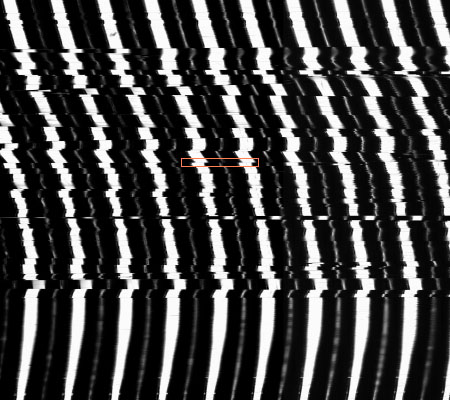
\includegraphics[width=0.9\textwidth]{images/brigance-cracks}
    \caption{General view (binned image).}
    \label{fig:brigcracks}
    \end{subfigure}
    \begin{subfigure}[t]{0.45\textwidth}
    \centering
    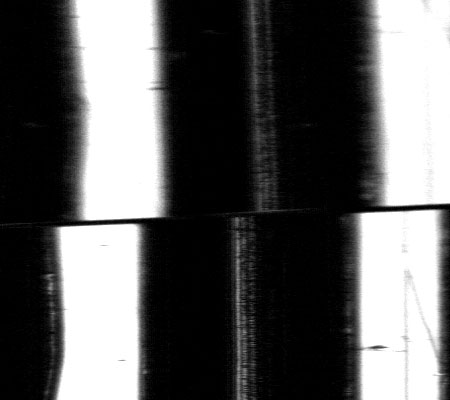
\includegraphics[width=0.9\textwidth]{images/brigance-crack-detail}
    \caption{Detailed view of a particular crack.}
    \label{fig:brigcrackdet}
    \end{subfigure}
    \caption{The Brigance disc as viewed from the RENE program.}
    \label{fig:brigdamage}
\end{figure}

We can clearly see from the binned image in \autoref{fig:brigcracks} many irregularities due to the cracks. However, the shifting is narrow and the general path to follow seems obvious. The detailed view in \autoref{fig:brigcrackdet} shows however that the crack is very thin, making it difficult to detect.

\subsection{Conclusion}

All provided samples are unique and show a lot of different properties according to the mediums and their condition. This means that a general solution for this problem is difficult to come up with. Some parameters will then probably have to be chosen to adapt the future solution to different types of medium. In the worst cases, the user intervention to help tracking the grooves may be mandatory.

\section{Summary}

This chapter presented an overview of the solutions developed at \gls{lbnl}. It covered the two systems, \gls{irene} and \gls{3dprobe}, both in terms of software and hardware. It also presented the common issues appearing while processing damaged audio records, and the test set provided by the laboratory with its specific properties. These samples will be used to test the new features.

The following chapters will cover the existing ways of figuring out these issues, and present new features implemented during this thesis to improve and ease the recovery of these damaged records.

\chapter{Manual tracking}
\label{chap:mantrack}

This chapter explains how we improved the manual tracking. Because there are a lot of different mediums and the same amount of issues coming with, it is not likely to find the best solution to solve each of them. There are some recordings to be recovered that have particular and unique issues, appearing only in a small section of the record. Likewise, some small artifacts can appear visually easy to catch and fix for the human eye, but very tricky to solve with a particular algorithm.

Therefore, for this kind of thing, falling back to a manual tracking can be the more appropriate solution.

\section{Current implementation}
\label{sec:mancurrentimpl}

As summarized in \autoref{chap:acqprocsys}, both \gls{rene} and \gls{prism} feature similar manual groove tracking. The system is simple but useful on specific cases. To start tracking, the user must select the proper option in the tracking options. When clicking on the general record view with the CTRL key pressed (left image on \gls{prism}), a first tracking point is stored. Then, each successive click adds a new point and a polyline is drawn connecting all previous points, giving the general track path as seen in \autoref{fig:mantrackprism}.

\begin{figure}[!ht]
\centering
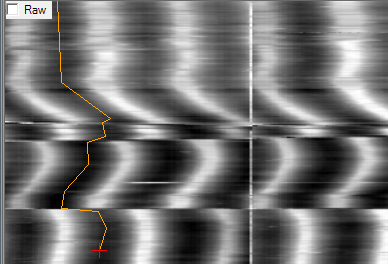
\includegraphics[width=0.5\textwidth]{images/manual-tracking-prism}
\caption{Manual tracking example in PRISM.}
\label{fig:mantrackprism}
\end{figure}

The program offers the possibility to store the tracked coordinates in a file to be used later. Finally, when the user applies the tracking, all points are interpolated and the processing step starts as usual.

\subsection{Limitations}

The current implementation is suitable to handle some complicated cases but suffers from several limitations:

\begin{itemize}
\item Unnatural way to draw a path over an image.
\item Tracking points can be manually put only on the binned (left) image, which can lack of precise information, especially if the scanned part is big and the record is cracked or damaged.
\item No possibility to undo parts already traced.
\item Tracking a whole record manually is a very slow process.
\end{itemize}

\subsection{Suggestions for improvement}

Regarding the previous limitations, several proposals were made at the project startup to find ways to improve the user experience and enhance the tracking efficiency.

\subsubsection{Touchscreen interface}

One of the concepts was to use a touchscreen interface. Nowadays, a lot of people are used to these interfaces such as tablets, smartphones, etc. Moreover, following a trace on a touch screen with the finger or a stylus seems to be user-friendly. This interface could also be convenient to re-align broken discs with shifted grooves (see \autoref{sec:issueshift}).

However, using a tablet would imply working on a specific operating system which would not be compatible with the current applications. It would be possible to implement a communication interface between the standard application and the UI but another problem could arise: these devices have mostly a limited capacity, while the amount of data processed for the sound recovery is very large. Nevertheless, using a simple touch screen within the current system and adapt the interface accordingly is still worth considering.

\subsubsection{Interactive tracking}
\label{sec:inttrack}

Another idea was to develop an \emph{interactive} way of tracking the grooves. The interface would display the groove scrolling \emph{continuously}, and the user would have to correct the lateral position to stay over the groove center.

The scrolling speed must be adaptable so that the tracking is convenient in different situations. Over areas where the surface is clean, it can be fast because there is no big correction to fix the track. When the right way is less obvious, the user can slow down and stop to choose the right way.

The zoom could also be adapted regarding of the speed. When the speed is slowed down, the zoom factor is greater to see precisely a specific part. When the speed is high, the user does not need to see the groove scrolling rapidly but should instead have an overview to stop at the next difficult point.

In fact, this feature could also be seen as a more entertaining way for this kind of work, because it could look like a ``game'' because of its animated and lively interface.

\subsubsection{Further improvements}

Beyond a brand new specific interface, other improvements to the user experience can be made to ease and accelerate the manual tracking.

The ability to undo what was done so far to be able to correct a wrong decision is a useful feature. Likewise, it could be gainful to be able to put some annotations before actually track the grooves. \gls{rene} and \gls{prism} already offer information and statistics about the scanned record. For example, one could notice that the signal on the graph between two shifted grooves is similar. It would then be possible to click on the specific ends to indicate that they are likely to be linked together for the tracking.

\subsection{Summary}

The current user interface for manual tracking is functional but can still be improved in many ways. The concept for a touchscreen interface is interesting but not easily applicable in the current state of the system. Therefore, the interactive method seems to be a good idea and its design and implementation is detailed in the next sections.

\section{Interactive tracking}

This section presents the interactive tracking feature as it has been integrated into the \gls{prism} program. The next subsections present it in terms of graphical interface, explain its utilization and detail its implementation.

\subsection{Graphical design}

\subsubsection{Location and integration}

As the current interface is already overflowed with all existing parameters and options, it is important to add the new feature so that it is integrated smoothly in the existing application, without making it tedious to use.

As seen in \autoref{fig:prismgui}, the interface is already able to show a detailed part of the disc on the right panel. When the user clicks on this detailed part, he can visualize other information on the signal. However, it is not designed to be interactive. In fact, each time the user selects a part on the right image, the corresponding part is reloaded and stored in a bitmap to be drawn on screen. The whole process is too time-consuming for an interactive drawing though it is suitable for its purpose.

The new feature has then to be separated from this detailed view. It has been chosen to put a tabbed panel to choose between the two configuration. As the user will not need both features at the same time, this is a suitable solution.

\subsubsection{Tracking panel}

The interactive tracking panel is separated in two parts: controls and visualization. The first part enables the user to manage and edit the different options while the second represents the record scan which the user has to follow to indicates the grooves. \autoref{fig:intpanelprism} represents the whole panel.

\begin{figure}[!ht]
\centering
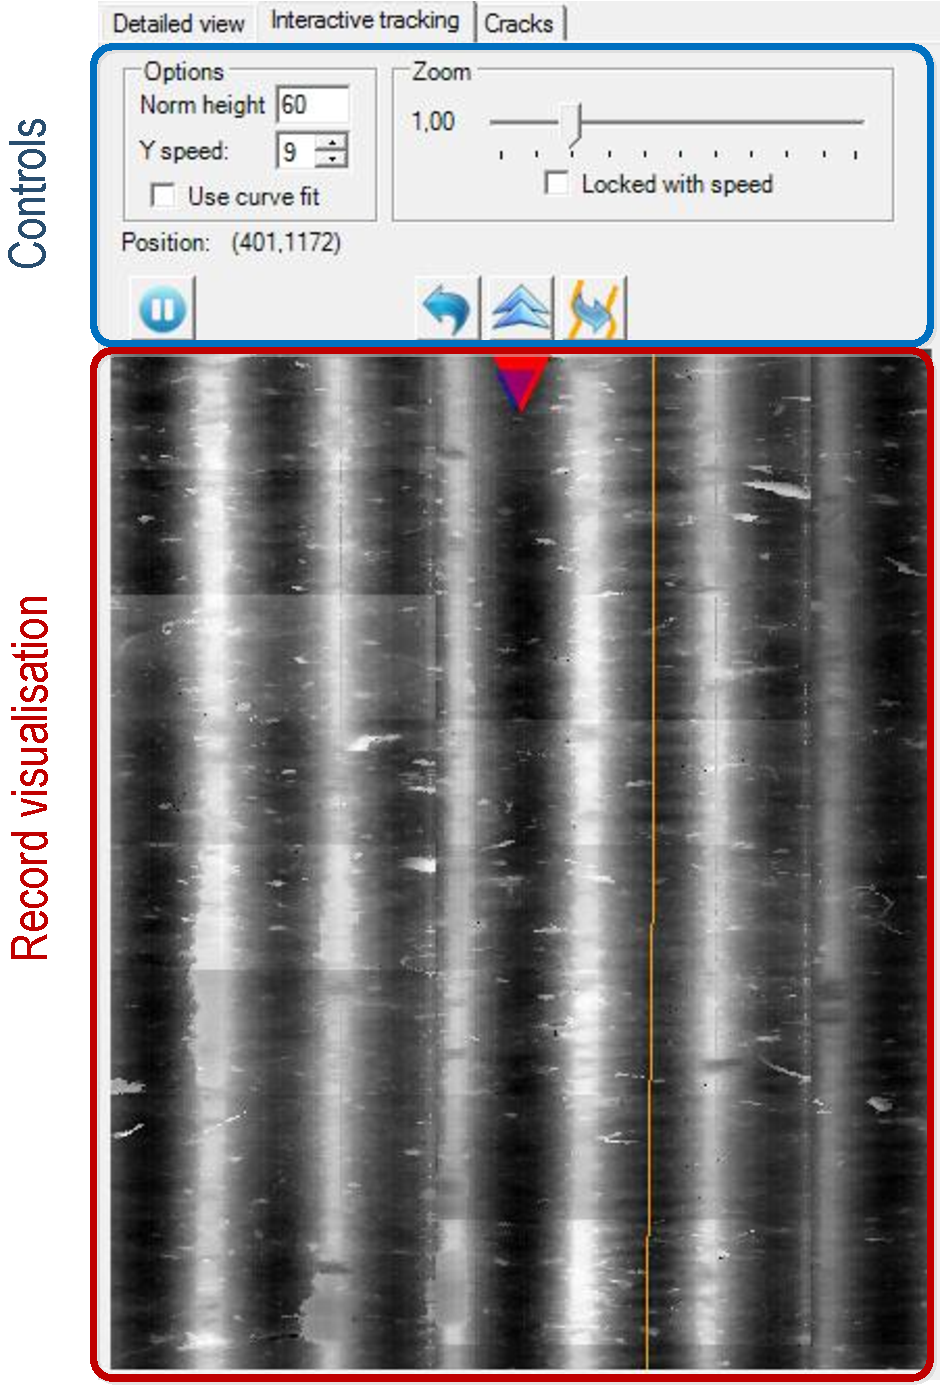
\includegraphics[width=0.6\textwidth]{images/int-track-panel-prism}
\caption{Interactive tracking panel in PRISM.}
\label{fig:intpanelprism}
\end{figure}

The controls enable to monitor the tracking by changing several parameters such as the speed or the zoom level. As explained in \autoref{sec:inttrack}, the zoom can also be locked regarding to the speed, using the corresponding option.

\subsection{Principle of operation}

To use the interactive tracking, the user first selects the corresponding button in the tracking options. Then, when the record is loaded, the corresponding disc is visible in the interactive panel. A red triangle acts as a beacon to clearly see the current tracked position.

When the user clicks on the panel and moves the cursor, the horizontal position moves accordingly. The goal is then to place the triangle tip on the center of the groove. While maintaining the mouse button pressed, the user may then increase the speed by using the mouse wheel. The record scrolls vertically while the horizontal position is still following the cursor.

To actually start the tracking, i.e. keep track of the points interpolated, the user must click the \emph{Play} button on the left.

\subsubsection{Synchronization between views}

The interactive view and the global view on the left are always synchronized. The current tracked position is visualized on the left panel of the application as a small red square and moves accordingly. When the tracking is performing, the corresponding polyline is drawn on the left part, as seen in \autoref{fig:intsynctrack}. The path is also represented in the right panel, so that the user is able to see which was the previous tracked groove before starting the next one.

\begin{figure}[!ht]
\centering
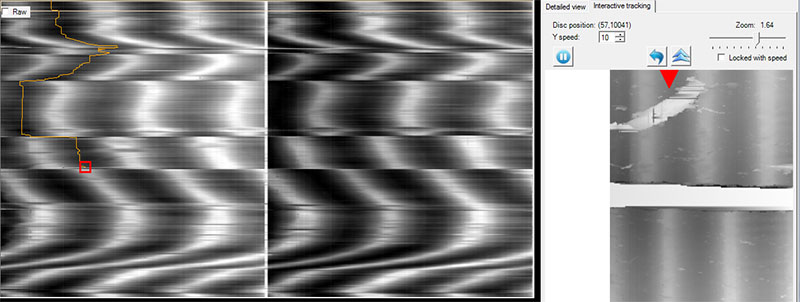
\includegraphics[width=0.9\textwidth]{images/int-track-sync}
\caption{Interactive tracking synchronized with the global view.}
\label{fig:intsynctrack}
\end{figure}

When the left panel is clicked, the position in the interactive panel is also changed accordingly. When the tracking is running (the \emph{Play} button is pushed), a click on the panel also has the effect of adding an interpolation point. In fact, this acts in the same way as the original manual tracking. It is useful for some areas where the disc is in good quality and passing through the entire groove interactively would be too long. The user can easily switch between the two alternatives while tracking a record.

\subsubsection{Undo option}

One of the problems that happens with the manual tracking is the lack of an option to undo the last actions. It appears quite frequently that the last action is improper resulting in a bad tracking. The interactive tracking offers the possibility to undo the steps up to the starting point.

\subsubsection{Groove center correction}

Another feature which has been added is the correction of the actual position to match the very center of the groove. In fact, the system is able to precisely find the groove center once the it is known which one is the current one to track. The user involvement is then more a way for helping the system to choose the correct groove from an approximated position.

The user will then see two triangles. A red one which is fixed and represents the position that the user points out, and the blue one which shifts to the deepest position in the surrounding area.

\subsection{Design and classes organization}

This part of the implementation is much about user interface and does not require a lot of processing. The main point is to find an appropriate way of integrating the new feature without blowing up the existing codebase which is already quite complex (see~\autoref{sec:prismarchi}).

The new feature has been implemented essentially in two new classes called \texttt{InteractiveControl} and \texttt{DrawPanel} as represented in the diagram of \autoref{fig:inttrackprismdiag}.

\begin{figure}[!ht]
\centering
\includegraphics{diagrams/int-track-prism.1}
\caption{Class diagram for the interactive tracking in PRISM.}
\label{fig:inttrackprismdiag}
\end{figure}

The first one embeds the whole control with the controlling part (toolbox) and the visualization path. It is a specific control and inherits the \texttt{UserControl} class of the WinForms \gls{api}. The specific interactive part drawing the record is handled by the second class. It inherits from the WinForms \texttt{Panel} class. Another class called \texttt{BeaconTriangle} has been created to simplify the rendering of the blue and red triangles indicating the tracked position.

The interactive panel is owned by the \texttt{frmMain} class already created in PRISM. It uses the \texttt{Hardware} class for the communication with the record information, e.g. to get the original bitmap or set the points building the tracking path. The reference to \texttt{PictureBox} called \texttt{pict} and \texttt{picture} point to the same instance. It represents the left panel showing the global view. The \texttt{InteractiveControl} class needs it to force the drawing when the values are updated (e.g. while points are being added).

An utility class called \texttt{Utils} stands for common operations used specifically for the new feature.

\subsection{Implementation details}

\subsubsection{Bitmap creation}

At creation, the scanned record must firstly be converted to a bitmap, so that it can be drawn on the panel. Most part of the process is implemented in the \texttt{BitmapFromData()} in the utility class.

As already explained, the raw data of the scanned record is stored as an array of floating-point values (see~\autoref{sec:3dcaptureprop}). They must then be converted and normalized to be stored as values in the range \numrange[range-phrase=--]{0}{255} to represents pixel values. The bitmap created has the \SI{8}{bpp} format, using a 256 colors palette of grayscale values, so that the memory is not wasted with other colors.

\subsubsection{Draw panel animation}

The main implementation point is to update and draw the panel. This part is handled using \gls{gdi}, provided in Microsoft .NET through the \texttt{System.Drawing} classes.

As its name implies, \emph{interactive} means to draw the objects several times per second, so that it is possible to output a smooth animation. The way WinForms are usually handled is not meant to perform animation. The panels are refreshed only when required, e.g. when a window has been hidden by another, or when it is resized to replace the components. To refresh the panel manually, it must be marked as invalid by calling the \texttt{Invalidate()} function.

To perform an animation, one may then use a \texttt{Timer} (provided in the \gls{api}) and, at each tick, update the view before invalidating the panel. The interval should be set to a value giving a high enough refresh rate. For example, with an interval of \SI{40}{\milli\second}, the corresponding refresh rate is $1/0.04 = \SI{25}{fps}$.

\subsubsection{Linear transformations}

Another important consideration is the transformations. Although there are not a lot of objects drawn on the panel, the correct positioning of all elements is the main point.

For example, the bitmap representing the record is placed regarding the user inputs. However, the relevant position is, from an external point of view, the coordinates in the record where the red triangle is pointing. On the other hand, from the drawing area perspective, the triangle is fixed at the top center. Therefore, to draw the bitmap at the correct location, the drawing coordinates must be inverted and shifted. When the targeted position is 30 pixels from the left and 200 from the top, the bitmap must in fact be translated by $(-30,-200)$ from the triangle tip.

There are different coordinate systems, as viewed in \autoref{fig:inttracktransfo}. Likewise, the zoom level influences the final position as well, and the final shift also depends on this factor.

\begin{figure}[!ht]
\centering
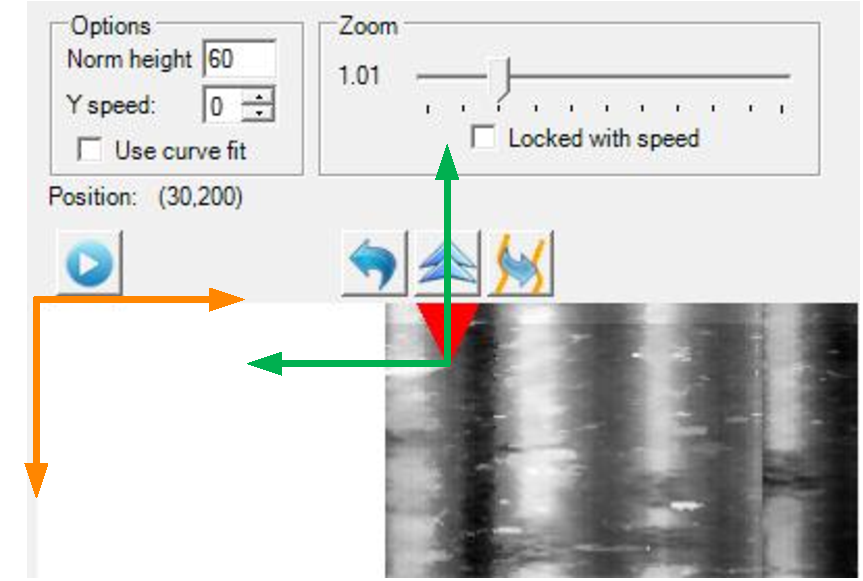
\includegraphics[width=0.6\textwidth]{images/int-track-transfo}
\caption[Panel and record coordinate systems in the interactive tracking panel.]{Panel and record coordinate systems in the interactive tracking panel. The first one is represented in orange and the second in green. When the record is drawn at $(30,300)$, the bitmap is translated to the left and top.}
\label{fig:inttracktransfo}
\end{figure}

In fact, each object has its own properties. To be properly drawn on screen, their position expressed naturally must be converted to the panel coordinate system. The needed transformations for each element are summarized in \autoref{tab:transforms}.

The most effective and flexible way to easily handle these conversions is to alter the global transformation matrix before rendering each object, instead of applying manually the transformations to the point. This enables to keep the position in their natural logical coordinates. The corresponding conceptual code is presented in \autoref{lst:inttransfo}.

\lstinputlisting[language={[Sharp]C},
caption={Interactive panel drawing and coordinate systems transformation.},
label={lst:inttransfo}]
{listings/interactive-panel.cs}

\begin{table}[h!]
\begin{center}
\tabulinesep=3pt
\begin{tabu} to 0.9\textwidth {| X[-1m] | X[m] | X[m] |} %{>{\bfseries}lX}
    \everyrow{\hline}
    \hline
    \rowfont[c] \bfseries
    Object & Coordinates relative to & Necessary transformations \\
    Record bitmap & position in the record where the user is pointing  & Inverse translation of the position \newline Scaling of the current zoom level \\
    Tracking path & position in the record of the points building the line & Idem as the bitmap \\
    Red triangle & top center in panel coordinates & Translation to the center of the panel \\
    Blue triangle & X: real tracked position in record coordinates \newline Y: fixed in panel coordinates & X: idem as the bitmap \newline Y: no transformation needed \\
\end{tabu}
\end{center}
\caption{Transformation of the different objects in the interactive panel.}
\label{tab:transforms}
\end{table}

Firstly, the actual panel coordinates are translated to the center of the screen and below the red triangle. This sets the new basis for the panel coordinate system, with the origin starting at the tip of the latter. This initial transformation matrix is saved to be restored later on.

The bitmap and the tracked points are drawn in the same coordinate system. One can note that for the bitmap, the inversion is not applied to the current matrix using a negative scale, but is manually set by defining the \texttt{renderPos} variable. This is to avoid that the bitmap is rendered as if it was flipped, which is not the desired behavior. We just want its starting position to be altered.

The matrix is then reset to draw the red triangle. No transformation is needed as it is directly positioned at the very top center. Then, to draw the actual tracked position indicated by the blue triangle, the same transformations as for the bitmap must be applied for the X coordinates. However, we cannot just alter the current matrix. Indeed, the zoom would alter the triangle size as well. As for the record, we only want the position to be altered. The only way is then to define a new matrix and only apply the transformation to the point, before setting the position.

\subsubsection{Groove center approximation}
\label{sec:centerapprox}

As explained in the previous section, the groove center is refined from the position indicated by the user. This is done by iterating $n$ points before and after the current point in the same row, and returning the deepest position. The $n$ value is determined using an approximated groove width and a tolerance factor $t$ in the range $[0,1]$. For example, if the groove width is $60$ and the tolerance $0.8$, then $n = \frac{60}{2} t = 24$.

The groove width can be fixed or determined by analyzing the record. This step will be explained in \autoref{sec:groovefilter}.

\subsection{Adaptation for RENE}

Although all the analysis was done in the \gls{prism} program, this feature is also useful for \gls{rene}, to recover very damaged discs acquired with the \gls{irene} 2D system. Most of the code implementing \gls{gui} was fairly quickly adapted for the program, as the custom controls deriving from the Windows Forms \gls{api} are directly reusable.

\subsubsection{Integration in the application}

In terms of user interface, the new interactive panel was added as a new tab on the left part, as viewed in \autoref{fig:ireneintgui}). The feature with the cursor following in the binned image as also been added. As almost all business logic is implemented directly in the \texttt{Form1} class, which also contains the sources of the main \gls{gui}, the code has been directly added in this class.

\begin{figure}[!ht]
\centering
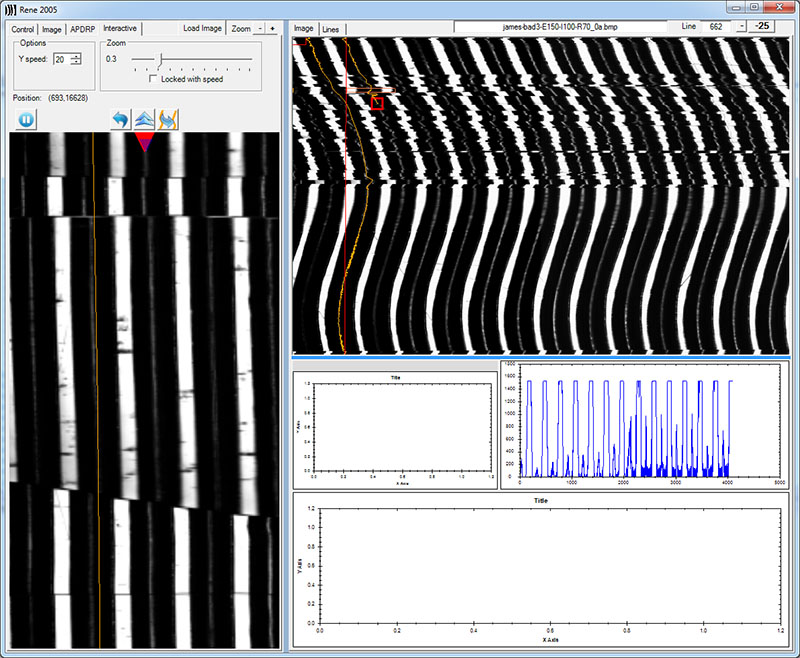
\includegraphics[width=0.9\textwidth]{images/int-tracking-rene}
\caption{Screenshot of the interactive tracking working in RENE.}
\label{fig:ireneintgui}
\end{figure}

\subsubsection{Groove center approximation}

The tracking step in \gls{rene} differs from the \gls{prism} implementation. In this case, the groove center is not already sought at this step, but instead the top edges delimiting a groove (the intervals as represented in \autoref{fig:irenegroove}). Then, in the processing part, the center is precisely found by looking inside the whole groove. However, while manually tracking a groove, the user does not trace both edges. Instead, he just highlights the approximate center, and the edges or computed by adding/subtracting a value conform to the groove width from this center. As the interactive tracking is based on the manual feature, the user will also follow the center.

Therefore, the main difference between \gls{rene} and \gls{prism} is how to approximate this center. In \gls{prism}, the real height can be used and it is straightforward to keep track of it by finding the lowest point in the neighborhood. In our case, to keep the real center, an optimal solution would be to detect the edge sides and find the center, in a way similar to what is already done for the processing step.

However, at this point, the tracking is just a rough approximation, and the real useful values are the top edges delimiting the groove. It will then be sufficient to keep track the brightest point in the neighborhood of the part pointed by the user to improve the tracking.

\subsubsection{Original image resizing}

An issue that appeared in \gls{rene} is that a single scanned ring loaded in the program has a huge resolution of \SI[product-units=single]{4096x80000}{px}. It appeared that handling the dynamic drawing of such a big bitmap, though feasible, was quite slow and made the tracking uncomfortable for the user.

The solution was to resize the original image before drawing it by a certain factor. After several tests, a factor of 8, resulting in a \SI[product-units=single]{512x10000}{px} image was sufficient.

\section{Finding grooves}
\label{sec:groovebot}

Another feature that can help the user while manually tracking a record is to highlight the groove bottoms at the start and the end of a revolution. Even if they are clearly seen as a lower intensity in \gls{prism} (and a lighter brightness with \gls{rene}), the match from the start and the end is not evident when a record is heavily cracked and then separated into pieces.

The main point for the user is then to correctly match the pieces together, while the tracking inside a piece itself could be easy enough to perform manually. The visual result will be the coloration of the groove bottoms with the same color sequence at the top and bottom of the binned view in the program. The result after implementation can be viewed in \autoref{fig:groovehighlight}.

\begin{figure}[!ht]
\centering
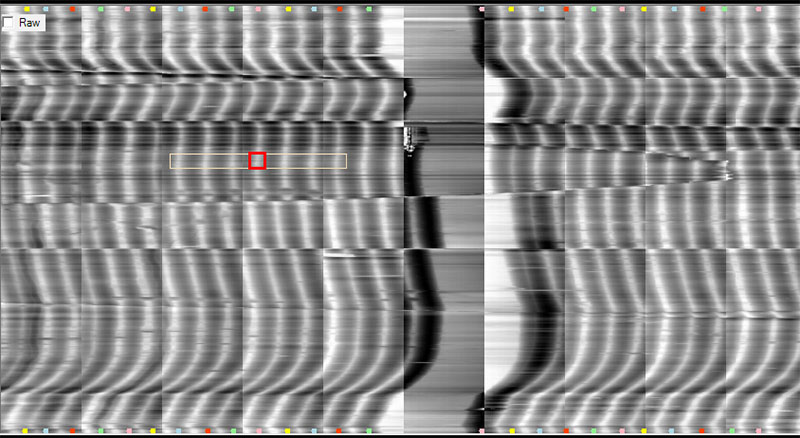
\includegraphics[width=0.9\textwidth]{images/groove-highlight}
\caption{Groove highlighting as implemented in PRISM.}
\label{fig:groovehighlight}
\end{figure}

Seeing the colored dots, the user then knows that if the track has the same color at the start than at the end, the tracking has a substantial possibility to be correct.

The techniques used to implement this feature will also be useful to detect groove for an automatic tracking system, to be able to reassemble them in a next step. This step will be explained in more detail in TODO. %TODO link section

\subsection{Finding groove bottoms}

The work is to find the groove bottoms on a given Y-position. The usual tracking methods (see~\autoref{sec:trackmethods}) do not need to find separate bottoms because once a groove is found, it can be followed until the end. This property is no more true on a damaged disc where the different parts can be shifted or even sometimes lost.

However, pointing out the position where the bottoms are located in a horizontal line is possible, using an adequate algorithm.

\subsubsection{Peak detection}
\label{sec:peakdetect}

The values on an horizontal line on a acquired record (mapping to a radial line on a disc and a line perpendicular to the grooves on a cylinder, see \autoref{sec:mapping}) can be seen as a one-dimensional signal showing grooves in a sectional view.

To find the groove bottoms on the signal, one cannot use the simple mathematical derivative because the signal is too noisy. A lot of variation can happen between two different values, because the signal is not smooth as if given by a simple mathematical function. One must then use a peak detection algorithm.

Different algorithms exist. For example, one can just smooth the signal by averaging it (low-pass filter) and then use the zero-derivate method. A simple well-suited method that does not alter the original signal is presented in \cite{peak12}. The idea is to define peaks and valleys. In fact, a peak is a location where the value is the highest between two valleys and a peak a location where it is the lowest between two peaks. A delta parameter defines the minimum Y distance between a peak and the next valley to really taking it into account.

\autoref{fig:graphpeakdet} presents a graph with examples values taken from the Bell disc and the points found by the algorithm.

\begin{figure}[!ht]
\tikzsetnextfilename{peak-detect-ex}
\centering
\begin{tikzpicture}
\begin{axis}[width=0.9\textwidth,unit vector ratio*=1 1 1]
%,xlabel=x,ylabel=value,xmin=0, xmax=2
\addplot +[mark=none] table[x expr=\coordindex,y=y] {graphs/peak-detect-ex.dat};
\addplot +[only marks, mark=*,forget plot, mark options={fill=red,draw=red}] table[x=xmin,y=ymin] {graphs/peak-detect-ex.dat};
\addplot +[only marks, mark=*, mark options={fill=green,draw=green}] table[x=xmax,y=ymax] {graphs/peak-detect-ex.dat};
\end{axis}
\end{tikzpicture}
\caption{Result of the peak detection algorithm.}
\label{fig:graphpeakdet}
\end{figure}

The algorithm first defines if it is looking for a maximum (peak) or minimum (valley). Then, by iterating through the data, it keeps track of the local minima and maxima. If at some point the height difference from the current point to the second one exceeds the defined delta, it means that a new extremum has been found. The point is then added and the state changed, before continuing the iteration.

The pseudocode of the algorithm is presented in \autoref{lst:peakdet}.

\lstinputlisting[language={[Sharp]C},
caption={Pseudocode of the peak detection algorithm.},
label={lst:peakdet}]
{listings/peak-detection.cs}

\subsection{Preparing data and filtering results}
\label{sec:groovepreparefilter}

This algorithm works very well on test data set, but in practice the acquired data is sometimes not clean enough. The previous algorithm enables to get rid of small noise but may still give false positives in some cases.

\subsubsection{Normalizing data}

The data range retrieved by the acquisition is not normalized. Given the record type, the acquisition parameters or other smoothing options in \gls{prism}, these values and their relative distance may vary a lot. Before finding the peaks on the data, the raw values must then be normalized so that the behavior remains the same regardless the situation. It was decided to normalize the values in the range $[\numrange[range-phrase=..]{0}{100}]$. This way, the minimum Y-delta chosen from the peak detection algorithm can be viewed as a percentage of the maximum delta between all values.

Also, as explained in \autoref{sec:3dcaptureprop}, the 3D sensor takes 180~points in a snapshot. This is also known as the number of fibers on the probe. Sometimes, it may happen that the beam is not exactly orthogonal to the record surface. This results in big differences between two snapshots that influence a lot the final shape. \gls{prism} already implements a feature known as Slope Correction. The user must enter manually a value representing the difference between the start and the end of a capture and the corresponding slope is subtracted from the original signal.

However, sometimes this correction is not sufficient. The slope is almost removed but the signal has not the same height between two snapshots and results in a ``staircase-shaped'' signal. The normalization is then not directly performed on the whole row, but in portions of the scan (180~points). This enables to smooth the signal and minimize the height differences.

The final pseudocode for the method \texttt{NormalizedRow()} can be found in \autoref{lst:normrow}.

\lstinputlisting[language={[Sharp]C},
caption={Pseudocode of the row normalization function},
label={lst:normrow}]
{listings/normalize-row.cs}

\subsubsection{Fix bad fiber}

Another problem that came in the first place was about bad fiber detection. The probe may have a manufacturing defect affecting one or two points (that remain the same) from all the 180 ones on the probe. Because the corresponding pixels will have the maximum possible value (as for bad points), they are always seen as whitish vertical lines on the image. In \gls{prism}, there is already a feature to remove a bad fiber. The user can enter a value from \numrange{1}{179} and the value is fixed by computing the mean from the two adjacent values.

However, the Bell disc has been acquired by the Library of Congress which possesses their own installation. It seems that it has two bad points at the border of the scan. This results in white lines at each scan borders, as seen in previous screenshots of this record from \gls{prism} (e.g. in \autoref{fig:intsynctrack} on the binned image).

The current implementation has two limitations: it cannot handle multiple bad fibers and cannot fix points from the border, as the mean of both values is used (at this time, only the 180~points of the current scan are known). An option has then been added to remove bad borders. The user can enter the number of bad fibers from the start or the end of the scan. Then, it simply overwrites the values from their neighbors inside the scan.

\subsubsection{Filtering results}
\label{sec:groovefilter}

Even with all the previous steps, there may still be some wrong values that come out from the peak detection. For example, in some situations with bad values, a groove may be detected twice. To avoid this, the filtering method analyzes the common distance groove size and ensures that the it is not too short, giving a tolerance factor.

The common distance is evaluated by the median of all distances between two consecutive points. This gives a pretty good estimation. Using the average would be badly influenced by uncommon distance, as seen for example in the middle of the scan in \autoref{fig:groovehighlight}. This value is also used for the interactive tracking, as viewed in \ref{sec:centerapprox}.

\section{Summary}

This part of the project ended with a new feature to the current system. The new interactive tracking enables to simplify the sometimes painful manual tracking. It provides a new way of tracking the grooves and several enhancements helping the operator to restore records. This feature is however not sufficient in practice, as in most cases the difficult part is to find the correct path when the record is cracked and the grooves possibly shifted.

The next chapter will present some ways to detect the cracks in a record. This will be a first step for the implementation of an automatic system to track damaged records, as well as a way of providing further information to the user for the manual tracking feature.

%\chapter{Automatic processing}

%\chapter{Chunk and groove detection}
\chapter{Towards an automated processing}
\label{chap:groovedetect}

The main problem to address in this project is that the current algorithms are unable to properly track (find) the grooves when a record is cracked.

This chapter will firstly summarize the current implemented tracking algorithms and explain why they cannot be used as such on cracked records. Then, it will explain a way of finding the cracks and distinguish the different pieces delimited by them. %Finally, the remaining work will be to find the grooves inside these chunks, in order to be able to track them later.
Finally, the remaining work will be to find the grooves inside these chunk, to track them and finally to reassemble all the pieces and construct the final track to be processed by the program.

\section{Existing tracking methods}
\label{sec:trackmethods}

\subsection{Tracking line}

One of the currently implemented automatic tracking method, called \emph{track line}, tries to find the approximate edges of a groove. It is especially used on disc records in \gls{rene}. This is achieved by finding the peaks in intensity and keeping track of the groove edges by detecting the changing intensity (as seen in \autoref{sec:reneprocessing}). Then, it follows the corresponding X-position scanning the record downward and adjusting it to the deepest value.

When the \emph{bottom} of the scanned record is reached, the tracking can simply continue at the top, meaning that a full revolution has been reached (see \autoref{sec:mapping}). The tracking is completed when the side of the record has been reached.

This method fails when there is just a little crack, because the depth is obviously completely wrong at this place, and the algorithm fails to find its way on the disc.

\subsection{Tracking depth}

The second method is the counterpart of the tracking line algorithm, operating in a similar way but specifically used for cylinders in \gls{prism}. The difference is that it tries to directly find the groove center instead of the edges. As the height values are expressively indicated by the 3D probe scanning, this can be done by looking for the deepest point in a local region of the record. The disc is then scanned downward the very same way as with the previous method.

\subsection{Tracking Fourier}

The second method uses a different approach. The binned image is scanned horizontally, giving the groove shapes for each row. Then, the Fast Fourier Transform algorithm is applied giving the frequency space of the signal. This enables to get the peak frequency and deduce the phase which gives the distance between two grooves. When the first groove has been tracked, the other ones can then be deduced by the computed phase.

This method works well when the records are not distorted, as the distance between two grooves remains invariable in the same row. Therefore, it is also inapplicable for cracked records for the same reasons.

\subsection{Conclusion}

The existing automatic tracking methods propose different ways which have proven to be effective for a large variety of records. However, this simple approach cannot be used anymore in the case of cracked records. The biggest issue is that when a crack appears, no information is relevant in the corresponding signal. It could be avoided until the damaged part ends up, but in this case the typical problem of shifting (see \autoref{sec:issueshift}) would make it almost impossible to follow correctly the good path.

Somehow, these cracks must be firstly detected in order to process the record correctly. The next sections explain ways to find cracks in the scanned records in order to distinguish the different pieces.

\section{Chunks detection}

As already seen in the previous sections we need a way to differentiate the pieces separated by cracks, which will now be called \emph{chunks} in the rest of this report. Rather than finding the cracks, the goal will be to find the chunks to be able to process them separately.

To detect them properly, a characteristic which differs in parts representing cracks and normal part of a record must be found. Then, some image processing algorithms must be applied in order to extract the contour of the chunk. These steps are explained in the next subsections.

\subsection{Cracked records characteristics}
\label{sec:crackrecchar}

The recording test set with specific damaged examples has already been presented in \autoref{sec:samplerec}. However, at this point, we need to investigate more deeply to find a way to clearly distinguish the cracks from the rest of a record.

For the records processed with \gls{3dprobe}, an early response to this problem is the information of the brightness intensity reflected by the probe, in order to see what looks like a crack in terms of brightness. This first example in \autoref{fig:crackdepthbri} comes from the Graham Bell disc.

\begin{figure}[!ht]
    \centering
    \begin{subfigure}[t]{0.45\textwidth}
    \centering
    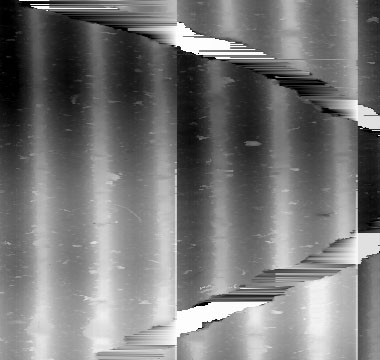
\includegraphics[width=0.9\textwidth]{images/bell-crack-raw}
    \caption{View of the heightmap.}
    \label{fig:crackdepth}
    \end{subfigure}
    \begin{subfigure}[t]{0.45\textwidth}
    \centering
    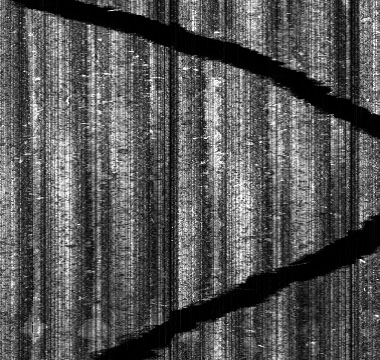
\includegraphics[width=0.9\textwidth]{images/bell-crack-bri}
    \caption{View of the brightness intensity.}
    \label{fig:crackbri}
    \end{subfigure}
    \caption{A crack in the Bell record visualized as depth and brightness intensity.}
    \label{fig:crackdepthbri}
\end{figure}

In \autoref{fig:crackdepth}, it is quite difficult to spot a clear difference. The crack area seems to be brighter but this is not very clear and some values seem to be erroneous. In fact, these peculiar values inside a chunk occur because of a feature implemented in \gls{prism}. When the acquired values of the beam are out of range, the probe return the maximum height value, normally appearing in white in the image. However, at loading time, the bad pixels detected as totally wrong are replaced by the weighted average of their neighbors. When a lot of bad points are detected, this results in these horizontal lines seen in \autoref{fig:crackdepth} making difficult to extract the cracks. This feature can be deactivated, making the cracks more visible in bright values, but also resulting in other bad points (not necessarily in cracks) not being fixed.

On the brightness image (\autoref{fig:crackbri}), the pixels appear much darker in the crack area. This happens in this case because the material of the underneath support reflects less brightness than the normal surface. Of course, in the general case the intensity depends on the material. For example, in a disc with metallic support, the brightness would be much higher instead. However, in all the samples used in this project from \gls{3dprobe}, the reflected brightness is clearly lower than the surface. This property will then be used to find the chunks.

\subsubsection{Differences with VisualAudio}

On the cracked discs processed by VisualAudio, the cracks are quite big and usually bigger than the actual grooves. The process to find cracks starts by decimating the image, e.g. by a factor of 16. The cracks detection can then be processed quickly.

However, in our case, the cracks appearing in wax cylinders and discs can be very small, usually smaller than an actual groove. If the image is binned, two much information is lost to properly find all cracks. The processing must then be applied on the original image. The size is bigger but this is not an issue with \gls{3dprobe}. Firstly, the scan is not separated in different files and has not to be merged. The resulting image is also smaller, as the number of points per line is smaller (see \autoref{sec:3dcaptureprop}) as well as the sampling frequency detailed in \eqref{eq:samprate3d}. The multi-pass scan is not an issue, as for vertically-cut records the passes are usually averaged instead of kept as individual values. Therefore, the final image size is not multiplied.

\subsection{Filtering}

When detecting a feature on a digitalized image, the first task is to apply a filter to eliminate the noise present in the image. What is typically needed is a way of smoothing (blurring) the image. Different filters can be applied to clean the source image.

\subsubsection{Convolution}

The mathematical operation for applying a filter is called a convolution (noted $\ast$). In the case of an image, the source can be viewed as matrix $A$. The new image is computed by applying a convolution matrix, also called \emph{kernel}, which contains different weights . To compute the new pixel value, the weighted sum of the current pixel and all the pixels around is calculated using the coefficients in the kernel.

\begin{equation}
\label{eq:convolsimple}
B =
\begin{bmatrix}
1/9 & 1/9 & 1/9 \\
1/9 & 1/9 & 1/9 \\
1/9 & 1/9 & 1/9
\end{bmatrix}
\ast A
\end{equation}

In \eqref{eq:convolsimple}, the $3 \times 3$ kernel results in a simple blur consisting of the average of all pixel values around. The dimensions of a convolution matrix must be an odd value but it is not necessarily square.

\subsubsection{Blurring types}

Other blurring types can be used depending on the desired results. A well-known filter is the Gaussian blur. Instead of using the same coefficients for every pixels, they are calculated using a Gaussian distribution in two dimensions. It is computed from the product of two Gaussians parameterized by $x$ and $y$. The corresponding formula is given in \eqref{eq:gauss2d}.

\begin{equation}
\label{eq:gauss2d}
G(x,y) = \frac{1}{2\pi\sigma^2}e^{-\frac{x^2+y^2}{2\sigma^2}}
\end{equation}

An example of a $5 \times 5$ kernel applying a Gaussian blur with $\sigma = 0.8$ is approximated in \eqref{eq:convolgauss}. The result is that the current pixel is much more weighted than the distant neighbors. The visual representation of the two dimensional Gaussian is viewed in \autoref{fig:convolgauss}.

\begin{equation}
\label{eq:convolgauss}
{\scriptsize
\begin{bmatrix}
0.0005 & 0.0050 & 0.0109 & 0.0050 & 0.0005 \\
0.0050 & 0.0521 & 0.1139 & 0.0521 & 0.0050 \\
0.0109 & 0.1139 & 0.2487 & 0.1139 & 0.0109 \\
0.0050 & 0.0521 & 0.1139 & 0.0521 & 0.0050 \\
0.0005 & 0.0050 & 0.0109 & 0.0050 & 0.0005 \\
\end{bmatrix}
}
\end{equation}

\begin{figure}[!ht]
\tikzsetnextfilename{gaussian-2d}
\centering
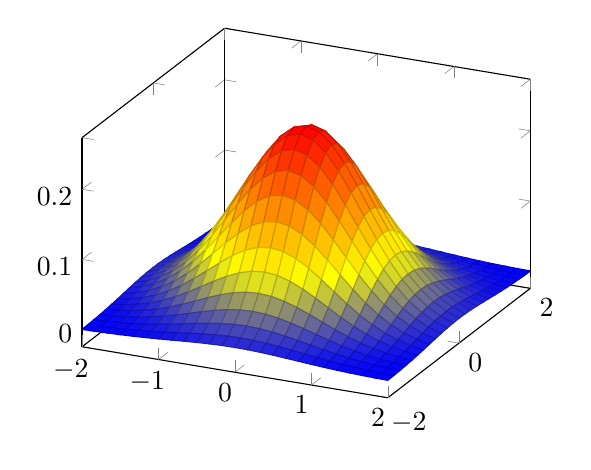
\begin{tikzpicture}
\begin{axis}[width=0.6\textwidth]
\addplot3[surf,domain=-2:2] {1 / (2 * pi * 0.8^2) * exp( -(x^2+y^2) / (2 * 0.8^2) )};
\end{axis}
\end{tikzpicture}
\caption{Visualization of the two-dimensional Gaussian with $\sigma = 0.8 $ .}
\label{fig:convolgauss}
\end{figure}

Another common filtering method is the median blur. The principle is slightly different than a convolution. Instead of computing a weighted sum, the new pixel value is computed by taking the median of the values selected by the kernel. It is no longer an averaging but a sorting operation. The selected value is thus an existing one and is less subject to degenerate pixels. The outcome is that the median filter preserves edges better than the other filters. The different filtering methods can be seen in \autoref{fig:filtermeth}.

All the filters in this example remove the noise in the image. The regular blur seems to remove information on the cracks while the Gaussian filter gives a better result (the crack edges are less blurred). The crack area is even better preserved with the median filter.

\begin{figure}[!ht]
\centering
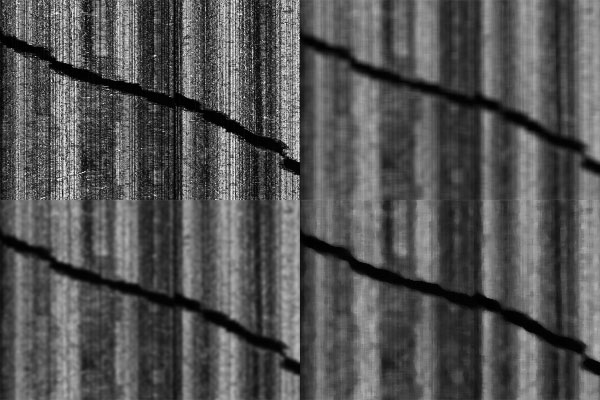
\includegraphics[width=0.9\textwidth]{images/filter-methods}
\caption[Visualization of the different filtering methods]
{Visualization of the different filtering methods with kernels of dimension $7 \times 7$. The top left part is the source image and on the right is the simple constant blur. The two bottoms parts are respectively the Gaussian and median filters.}
\label{fig:filtermeth}
\end{figure}

\subsection{Segmentation}
\label{sec:chunksegm}

Once the noise is removed in the source image, the next step is to segment the image. This process groups the pixels with common properties that we want to keep as valuable information (commonly called the object), and distinguishes them from the rest (the background). In this case, we want to keep the chunks areas and remove the cracks.

\subsubsection{Histogram}

A common tool helping for the segmentation operation is the histogram. A histogram represents the statistical distribution of a variable. Therefore, computing the histogram of an image means to compute the number of occurrences of each pixel values (usually in the range \numrange[range-phrase=--]{0}{255} for a bitmap). In our case this corresponds to the brightness intensity.

The histogram of a portion of the brightness image from a cracked disc can be seen in \autoref{fig:histocrack}.

\begin{figure}[!ht]
\tikzsetnextfilename{histo-crack}
\centering
\begin{tikzpicture}
\begin{axis}[width=0.7\textwidth,xlabel=Intensity value,ylabel=Frequency]
\addplot +[mark=none, fill=blue] table[x expr=\coordindex,y=y] {graphs/histo-crack.dat};
\end{axis}
\end{tikzpicture}
\caption{Histogram of a cracked record portion.}
\label{fig:histocrack}
\end{figure}

This histogram shows clearly different peaks on the intensity value. The first peak represents very dark pixel values. As predicted, this is the intensity inside the crack area, which is clearly detached from the rest of the image. The cracks is approximately represented by the intensity between \numrange[range-phrase=--]{0}{10} and the rest of the image in the intensity \numrange[range-phrase=--]{11}{255}.

\subsubsection{Thresholding}

With the histogram, we have the information to separate the regular record surface from the cracks. The thresholding is one of the existing methods to segment the image. It simply consists of creating a binary image from a defined threshold. If the pixel value in the source is smaller than the threshold, the destination will get the value 0. Otherwise, it will get the value 1 (in practice, often the maximum intensity value, e.g. 255 for a byte-depth bitmap), as summarized in \eqref{eq:thresh}.

\begin{equation}
\label{eq:thresh}
\dst(x, y) =
\left\{
\begin{array}{l l}
    1 & \text{if } \src(x, y) > \text{thresh},\\
    0 & \text{otherwise}.
\end{array}
\right.
\end{equation}

\autoref{fig:threshex} shows the result of the thresholding applied on a portion of the Bell record.

\begin{figure}[!ht]
\centering
    \begin{subfigure}[t]{0.45\textwidth}
    \centering
    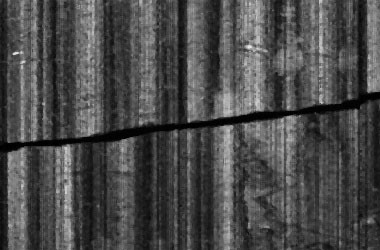
\includegraphics[width=0.9\textwidth]{images/thresh-before}
    \caption{Before the thresholding (grayscale image).}
    \label{fig:threshbef}
    \end{subfigure}
    \begin{subfigure}[t]{0.45\textwidth}
    \centering
    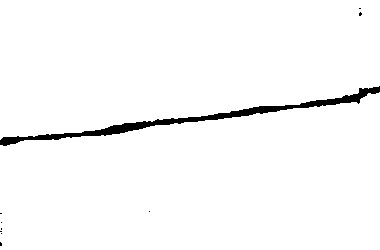
\includegraphics[width=0.9\textwidth]{images/thresh-after}
    \caption{After the thresholding (binary image).}
    \label{fig:threshaft}
    \end{subfigure}
    \caption{Result of the thresholding operation on a portion of a cracked record.}
    \label{fig:threshex}
\end{figure}

The crack is well separated from the rest of the surface, except for some small artifacts in the top right and bottom left of the binary image. The methods to get rid of the latter will be explained in the next section.

\subsubsection{Brightness normalization}
\label{sec:brinorm}

Another way to improve the cracks detection will be to normalize the brightness signal. The raw information from the probe might indeed not be constant for every 180 points in a pass. Likewise, on the histogram example of \autoref{fig:histocrack}, it seems that the the range in the intensity values is not entirely used. The maximum around 180. This explains why the brightness image looks quite dark.

In fact, \gls{prism} already implements a function normalizing the brightness in the vertical direction. Each captured points on the whole record are then rescaled from their specific properties.

The implemented algorithm computes a histogram for each column of the record. Then, in each of these, it iterates downward from the last intensity and stops when $\frac{4}{10}$ of the brighter pixels are reached. The most represented intensity (peak) in this portion is stored and then all values in the corresponding column are divided by its value. This results in a loss of information for the brighter (but underrepresented) values while the whole normalized image will be brighter and better emphasize the difference from lower and middle intensities. The visual result of the algorithm is visualized in \autoref{fig:brinorm}.

\begin{figure}[!ht]
\centering
    \begin{subfigure}[t]{0.45\textwidth}
    \centering
    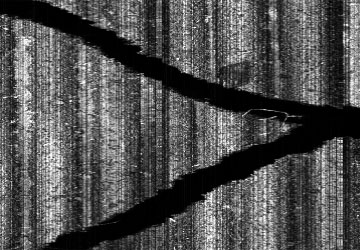
\includegraphics[width=0.9\textwidth]{images/bri-norm-before}
    \caption{Without normalization.}
    \label{fig:brinormbef}
    \end{subfigure}
    \begin{subfigure}[t]{0.45\textwidth}
    \centering
    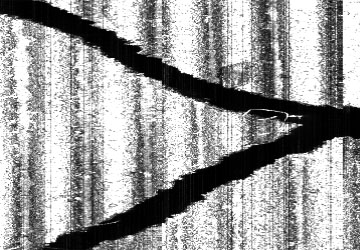
\includegraphics[width=0.9\textwidth]{images/bri-norm-after}
    \caption{With normalization.}
    \label{fig:brinormaft}
    \end{subfigure}
    \caption{Result of the brightness normalization in PRISM.}
    \label{fig:brinorm}
\end{figure}

The cracks is more evidently visible in the normalized image. Some artifact are now visible in the crack itself, as the range is greater. The threshold must then be adapted when working with normalized brightness.

Using this feature will be interesting in cases where the threshold can hardly differentiates the object from the background.

\subsection{Cleaning}

The thresholding which segments the object from the background only takes into account the value of a single pixel to decide if it is part of a chunk or a crack. In practical cases, the distinction is almost never that evident. The histogram of an image shows peaks as statistical information but the final chosen threshold is a compromise to separate at best the two parts. There will then be some background pixels considered as being part of the object and vice versa. One possibility to clean these regions is to use the morphological operations.

\subsubsection{Morphological operations}

Morphological operations are a technique to clean an image based on the pixels in the neighborhood. These are then boolean masks applied on the binary image in a way similar to the filtering operations seen before.

As the coefficients are 0 or 1, a mask is usually defined by its shape and is called a \emph{structured element} in this context. A typical shape is the cross, as defined in \eqref{eq:morphocross}.

\begin{equation}
\label{eq:morphocross}
M =
\begin{bmatrix}
0 & 1 & 0 \\
1 & 1 & 1 \\
0 & 1 & 0
\end{bmatrix}
\end{equation}

The mask $M$ is evaluated on each pixel as a common filter. The result is then the number of pixels contained in the cross shape.

The two basic operations using these structuring elements are called erosion and dilation. If $n$ is the number of pixels from the structuring elements, these operations $E$ and $D$ are defined as in \eqref{eq:morphoop}.

\begin{equation}
\label{eq:morphoop}
\dst(E) =
\left\{
\begin{array}{l l}
    1 & \text{if } n = 1,\\
    0 & \text{otherwise}.
\end{array}
\right. \qquad
\dst(D) =
\left\{
\begin{array}{l l}
    1 & \text{if } n > 1,\\
    0 & \text{otherwise}.
\end{array}
\right.
\end{equation}

The first one removes some pixels from the object and the second one add pixels to the object. These operations are most often applied together. Performing a dilation on an erosion ($E \to D$) is called an opening and the inverse ($D \to E$) a closing.

\subsubsection{Results}

Which operation to use depends on the context. The opening removes small regions considered as the object that are smaller than the structuring element. Closing adds small parts in the object that were considered as background, i.e. it ``closes the holes''.

The example in \autoref{fig:morphoex} shows the difference after applying a closing on a segmented binary image from a cracked record. In this case, the erosion and dilation elements are both $3 \times 3$ and each of them is applied five times (in 5 passes).

\begin{figure}[!ht]
\centering
    \begin{subfigure}[t]{0.45\textwidth}
    \centering
    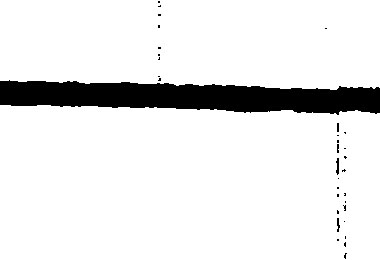
\includegraphics[width=0.9\textwidth]{images/morpho-before}
    \caption{Initial binary image.}
    \label{fig:morphobef}
    \end{subfigure}
    \begin{subfigure}[t]{0.45\textwidth}
    \centering
    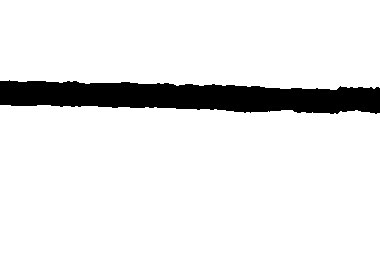
\includegraphics[width=0.9\textwidth]{images/morpho-after}
    \caption{After the operation.}
    \label{fig:morphoaft}
    \end{subfigure}
    \caption{Five passes closing to eliminate black pixels in the chunks.}
    \label{fig:morphoex}
\end{figure}

\subsection{Contours extraction}
\label{sec:contextract}

Finally, when the chunks are separated from the cracks, the remaining work is to extract the contours, which will define and distinguish all the chunks in the record. The output of this step is a list of polygons (itself a list of points), describing the contours of each chunks.

The standard behavior is to describe every pixel of the contour in the image. However, one step further is to approximate a simple polygon from this set of points, as viewed in \autoref{fig:contourapprox}. This enables to remove small noise from the contours detection and lighten the storage.

\begin{figure}[!ht]
\centering
    \begin{subfigure}[t]{0.45\textwidth}
    \centering
    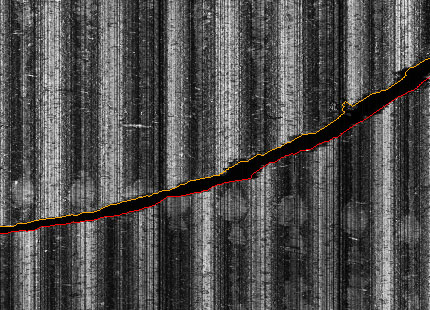
\includegraphics[width=0.9\textwidth]{images/approx-without}
    \caption{Without polygon approximation.}
    \label{fig:withoutapprox}
    \end{subfigure}
    \begin{subfigure}[t]{0.45\textwidth}
    \centering
    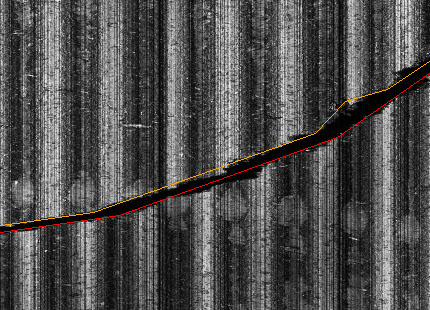
\includegraphics[width=0.9\textwidth]{images/approx-with}
    \caption{Using polygon approximation.}
    \label{fig:withapprox}
    \end{subfigure}
    \caption{Illustration of the contour detection and approximation.}
    \label{fig:contourapprox}
\end{figure}

\subsection{Tests and results}

The previous sections explained the techniques to implement the chunks detection. As this step implies a lot of experimentation to properly find the best parameters to use, a separate application has been written enabling to easily visualize the results and change all parameters. This enables to test quickly the best parameters to use for a proper detection, without the overhead of loading a whole acquisition using \gls{prism}.

\subsubsection{Cracks detection application}

This application has been written in \Csh{} in order to simplify the integration into \gls{prism}. Also, for the image processing algorithm, the OpenCV library (more precisely its \Csh wrapper called Emgu CV) has been used. Almost all techniques and algorithms detailed in the sections above are implemented in an efficient way in this library.

The program loads directly pictures from the filesystem. For the early tests, some parts of records have been loaded into \gls{prism} and saved as pictures. A screenshot of this program is presented in \autoref{fig:crackdetprog}.

\begin{figure}[!ht]
\centering
\includegraphics[width=0.9\textwidth]{images/crack-test-prog}
\caption{Screenshot of the cracks detection test program.}
\label{fig:crackdetprog}
\end{figure}

The four steps explained in the previous section are visualized in the program. This enables to clearly see the results for each steps separately and decide how to change parameters to improve the final detection. The four images scroll together be able to easily compare the results.

At the beginning, several edge detection algorithms have been tested, e.g. the well-known Sobel and Canny filters. In the end, they were not suitable for our purpose. The thresholding detailed in \autoref{sec:chunksegm} is the only algorithm that has been implemented in \gls{prism}.

\subsubsection{General results}

In general, most of the cracks are easily detected by correctly adapting the different parameters. However, others are really hard to detect, when they are very tight. Fortunately, when it is the case there is normally no groove shifting. This means that some cracks can be avoided. As the system is quite different from VisualAudio, this will not cause a problem on the tracking. If the image is binned by a factor of 30, any crack being smaller than around 10 pixels is not even spotted by the tracking algorithm.

The main issue will be when a crack is not entirely detected. The frontier of the chunk can stop anywhere, as seen in \autoref{fig:crackbellprob} causing future linking problems.

\begin{figure}[!ht]
\centering
\includegraphics[width=0.8\textwidth]{images/crack-bell-prob}
\caption{A very thin crack not entirely detected on the bell disc.}
\label{fig:crackbellprob}
\end{figure}

In VisualAudio, even if the cracks are much bigger, this issue can also happen. The workaround is to manually edit the exported image to ``draw'' the missing part. In the case of \gls{prism}, we will try to avoid it, and the frontier detection as explained in \autoref{sec:findfrontiers} should not be affected by this issue.

\subsubsection{Bell disc}

On the bell disc, some cracks are easily detected while others are really hard to spot. The following parameters gave good results.

\begin{itemize}
\item Not using brightness normalization
\item Using $3 \times 3$ median blur
\item Threshold of 20
\item 5 passes opening morphology (TODO kernels)
\item Bad fibers: two bad fibers at the start of each capture
\end{itemize}

Using the brightness normalization as seen in \autoref{sec:brinorm} does not really change the results with an adapted threshold.

\subsubsection{Dickson cylinder}

As described in \autoref{sec:samplerec}, this record contains also some parts where the wax layer is broken and no groove is visible. Apart from this, a single radial crack crosses the whole record at the beginning. This crack is easy to detect as it is wide. At some point the crack is getting tighter and difficult to distinguish from the rest of the record. It is however in a very damaged part where the grooves are very difficult to distinguish as well, even for a human.

The parameters do not influence a lot the detection and will then remain the same as for the Bell disc above. It would be possible to extract several parts of it but probably not entirely automatically.

%TODO parameters
%bad fiber: two bad fibers at the start of each capture

\subsubsection{Boas cylinder}

For this record, the brightness normalization must be used, because the range of intensity is far bigger than with other records, making the cracks almost invisible if not used. The final threshold to use is then greater than for the other records.

On this particular acquisition the height between different chunks varies also a lot. This should however not interfere with the detection and tracking of grooves as it will be done separately between the different chunks. A more troublesome issue is that with these parameters, some small regions are detected as chunks. The code will handle this by removing too small areas, but the final tracking and linking steps will be probably very difficult on some parts.

\begin{itemize}
\item Using brightness normalization
\item Using $3 \times 3$ median blur
\item Threshold of 80
\item 5 passes opening morphology with $3 \times 2$ for erosion and $2 \times 2$ for dilation
\item Bad fibers: one bad fiber at the end of each capture
\end{itemize}

Regarding all the issues from this particular record, it seems that it will be a better candidate for the manual and interactive tracking features, at least for some parts of the record.

\subsection{Design and integration into PRISM}

Almost all the implementation of the automatic tracking feature has been done in the namespace and folder \texttt{prism.CracksProcessing}. This way the specific code is easily localizable. The schema with the new added objects is represented in \autoref{fig:chunksdetectdiag}

\begin{figure}[!ht]
\centering
\includegraphics{diagrams/chunks-detection.1}
\caption{Class diagram for chunk detection.}
\label{fig:chunksdetectdiag}
\end{figure}

Firstly, the \texttt{ChunkDetector} class contains all processing code related to chunk detection. Most algorithms use Emgu CV for the specific step. From the user's point of view, the only interesting method is \texttt{Process()} which will analyze the loaded record and return a list of chunks. The constructor takes in parameters the \texttt{Hardware} object representing the record.

A chunk is itself described in its own class named \texttt{CrackedChunk}. The contour of the chunk can be accessed via the property Contour. The rest of the implementation will be explained as other properties are added.

The way all the parameters (thresholding, number of passes, etc.) will be explain more generally in TODO.

\section{Establishing frontiers}
\label{sec:findfrontiers}

At this stage of the processing, a collection of objects describing a physical chunk has been computed. It consists of a list of points describing a simple polygon (a polygon without intersecting lines). However, this polygon can still be non-convex. In the general case, it could be a non-trivial shape.

This section explains how to separate a chunk into several \emph{frontiers} which will be the starting point for the groove detection and the tracking.

\subsection{Difference with VisualAudio}

At this point, the choice has been made not to directly follow the idea of VisualAudio. In the latter, the next step after the chunks detection is directly the tracking (or even processing, as there is no previous tracking step as with \gls{irene}). The portion inside the chunk is isolated by applying a mask, and the grooves are found and tracked by a method using histograms (see Chapter~6 in \cite{seydoux08}). It is only after this step that the chunks (now defined by a set of traces, or grooves) are separated in frontiers to continue towards the linking step.

This choice was made after analyzing the VisualAudio code and documentation. This part was quite complex and it required some algorithms that did not look relevant in the case of \gls{prism}. Instead, it was decided to geometrically separate the chunk into frontiers, before finding and tracking the groove from the detected frontiers.

\subsection{Goal of this step}
\label{chap:linking}

To correctly link the trace, it is mandatory that the different pieces to link are convex or, more precisely, at least monotone in respect to the horizontal axis\footnote{A polygon monotone in respect to a line $L$ means that every line parallel to $L$, in this case the x-axis (horizontal), intersects the polygon no more than twice.}. As the grooves are scanned vertically from the acquisition, it is not a problem if the concavity appears on the horizontal direction. However, in the case of a chunk as illustrated in \autoref{fig:chunkdef}, it looks obvious that the grooves on the left part are split by the frontier. A missing part of these grooves are located in another part of the record.

\begin{figure}[!ht]
\centering
    \begin{subfigure}[t]{0.45\textwidth}
    \centering
    \includegraphics[width=0.9\textwidth]{images/chunk-concave}
    \caption{The initial chunk.}
    \label{fig:chunkdef}
    \end{subfigure}
    \begin{subfigure}[t]{0.45\textwidth}
    \centering
    \includegraphics[width=0.9\textwidth]{images/chunk-zones}
    \caption{The same chunk separated into zones.}
    \label{fig:chunkzones}
    \end{subfigure}
    \caption[Visualization of a non-convex chunk.]
    {Visualization of a non-convex chunk. The blue lines represent the grooves inside the chunk.}
    \label{fig:chunkconcave}
\end{figure}

In fact, the problem can be solved by splitting the chunks into well-defined parts. In VisualAudio, these parts are called \emph{zones}. The corresponding zones from the previous example can be seen in \autoref{fig:chunkzones}. With this separation into zones, the tracking of grooves inside each zone is no more problematic.

This separation looks evident for the human eyes, but the exact definition is more difficult to spot. We must firstly define what is a frontier.

\subsubsection{Frontier definition}

A frontier is either at the top or the bottom of a chunk. A top frontier has only some content of a chunk below line, while a bottom frontier has only some content above. A convex-shaped chunk has then only one top frontier and one bottom frontier. \autoref{fig:chunkfrontiers} visualizes the frontiers of the previous non-convex chunk.

\begin{figure}[!ht]
\centering
\includegraphics[width=0.6\textwidth]{images/chunk-frontiers}
\caption[The chunk with highlighted frontiers.]
{The chunk with highlighted frontiers. The three zones are defined by the common top and bottom frontiers.}
\label{fig:chunkfrontiers}
\end{figure}

A property is that if there is $n$ top frontiers in a chunk, there is also $n$ bottom frontiers. The zones are then defined by a common top and bottom frontier of a chunk. Of course, one of the two may be smaller but a single zone is always only between the mingled part of these frontiers. The next step is to find an algorithm to extract the frontiers.

\subsection{Frontier extraction}

\subsubsection{Detection}

%From what has been found interesting point to separate them 
To extract the frontiers, an analysis of the horizontal variation of the shape must be done. Indeed, as explained at the beginning of this section, we are looking for pieces monotones in respect to the x-axis. A simple algorithm is then to iterate through all the points of the shape and detect the changes in direction. If the points are listed in a counterclockwise rotation, the X coordinates for bottom frontiers are increasing, respectively decreasing for top frontiers.

Whenever the X direction changes, a new frontier is detected. This method is visualized in \autoref{fig:frontierdet}.

\begin{figure}[!ht]
\centering
\includegraphics[width=0.6\textwidth]{images/frontier-detect}
\caption{Frontier detection based on horizontal variation.}
\label{fig:frontierdet}
\end{figure}

The corresponding algorithm is pretty simple to implement. To avoid that a single frontier is detected separately, the iteration must start at either the leftmost or rightmost point of the shape.

\subsubsection{Improvement}

The solution explained above is not sufficient in practical cases. A chunk is not necessarily smooth-shaped, but may comport several local modifications that mean no real change of direction. This problem can be minimized with the polygon approximation (already implemented as part of the chunk detection, see \autoref{sec:contextract}), but even in this case some wrong results are possible.

In fact, we want to define a new frontier that has a defined minimum length, i.e. when the delta (in X coordinate) between the current position and the local extremum of the current frontier is large enough. Then, the previous frontier stops at the last extremum and the current one starts at the same location.

Actually, this algorithm has already been discussed and is the peak detection algorithm (see \autoref{sec:peakdetect}). \autoref{fig:frontierdetalgo} demonstrates the relation between the peak and frontier detection on an example. In \autoref{fig:frontierdet2}, the graph corresponds to the X coordinates of the polygon points plotted from the leftmost one.

\begin{figure}[!ht]
\centering
    \begin{subfigure}[b]{0.45\textwidth}
    \centering
    \includegraphics[width=0.9\textwidth]{images/chunk-peaks}
    \caption{Chunk with frontiers extremities.}
    \label{fig:frontierdet1}
    \end{subfigure}
    \begin{subfigure}[b]{0.45\textwidth}
    \tikzsetnextfilename{frontier-detect}
    \centering
    \begin{tikzpicture}[scale=0.9, baseline]
    \begin{axis} [every node near coord/.style={font=\sf,text=black},
    %[width=0.9\textwidth,
    %unit vector ratio*=1 0.3 1
    ]
    %,xlabel=x,ylabel=value,xmin=0, xmax=2
    \addplot +[mark=none] table[x expr=\coordindex,y=y] {graphs/frontier-detect.dat};
    
    \addplot +[only marks, mark=*,forget plot, mark options={fill=red,draw=red},
    nodes near coords, point meta=explicit symbolic
    ] table[x=xmin,y=ymin,meta=valuemin] {graphs/frontier-detect.dat};
    
    \addplot +[only marks, mark=*, mark options={fill=green,draw=green},
    nodes near coords, point meta=explicit symbolic
    ] table[x=xmax,y=ymax,meta=valuemax] {graphs/frontier-detect.dat};
    \end{axis}
    \end{tikzpicture}
    \caption{Plot of the chunk X-coordinates.}
    \label{fig:frontierdet2}
    \end{subfigure}
    \caption[Relation between peak and and frontier .]
    {Relation between peak and and frontier detection inside a chunk. The extremities of each frontiers are numbered in both cases and correspond to the extremums on the resulting signal (right side).}
    \label{fig:frontierdetalgo}
\end{figure}

It is clear that the frontier extremities are defined by the peaks and valleys in the corresponding signal. Bottom frontiers are located between a peak and a valley in this order and top ones between a valley and a peak.

One can note that the chunk is previously polygon approximated (the whole shape is described with 28 points).

\subsubsection{Final algorithm}

The peak detection algorithm does the main work of finding the extremities. From these values, it remains to extract the different frontiers. In the easiest case, when the chunk is convex, the detection will return one maximum and no minimum. The unique bottom frontier is then located between the left-most point to the maximum, and the top one from the maximum to the end.

The pseudocode in \autoref{lst:frontierex} presents the final algorithm.

\lstinputlisting[language={[Sharp]C},
caption={Pseudo for the frontier extraction, using the peak detection algorithm.},
label={lst:frontierex}]
{listings/frontier-extract.cs}

The \texttt{FindFrontiers()} function firstly finds the left-most point and stores its index. Then it copies the X coordinates of all points starting by this index in \texttt{pointsX}. The peak detection is applied on this array. Finally, the corresponding frontiers are created from the found extremities. In the for loop are found the possible mid frontiers.

The \texttt{AddNewFrontier()} function simplifies the storage of the results, separating the top frontiers from the bottom ones. It also verifies that the frontier has a minimal size before adding it to the corresponding collection.

\subsection{Interpolation}
\label{sec:frontierinterp}

At this point, we have a collection of frontiers per each chunk. To have all information available for future steps, another task must be applied: the interpolation of the frontier border. For the moment, the list of points defining the border has only the property of being defined from the left-most point to the right-most point of the frontier. However, following the definition of a frontier and the algorithm used for its detection, a small change of direction may still occur within the frontier, possibly resulting in several points with the same X coordinate in different values. Moreover, as the border may have been approximated (see \autoref{sec:contextract}), the distance between two points is not defined.

More theoretically, we need a mathematical discrete function that is defined from the left to the right point, with the standard definition that for each input X, only one output Y is defined. The border must then be interpolated in the horizontal direction.

\subsubsection{Linear interpolation}

As the list of points defines a well-approximated polygon, we can directly use a linear interpolation. The basic algorithm is given in \autoref{lst:lininterpol}.

\lstinputlisting[language={[Sharp]C},
caption={Basic linear interpolation algorithm.},
label={lst:lininterpol}]
{listings/lin-interpolation.cs}

The main formula is on lines 15 and 16, where the point is created. The X coordinate is directly the consecutive one and the Y is computed by interpolating the two out points. This algorithm is simple but not sufficient. As already said, it is possible that two points have the same value. This algorithm crashes when it happens because of a division by zero on line 16 (\texttt{x2 - x1}). A condition must be added between before the inner loop to ensure that \texttt{x1} is different than \texttt{x2}. If the horizontal distance between two points is null, there is no need to interpolate between these ones.

Moreover, the strict order is not implied and two non-consecutive points may appear on the same vertical line. This would give wrong results for the interpolation. A solution to ensure the correct result is to use a proper data structure, as a sorted dictionary with the key corresponding the X position. This ensures the two properties, order and uniqueness.

\subsubsection{Final algorithm}

With the last additional changes, the algorithm is functional but may still be improved. In an extreme example, e.g. as the one previously seen in \autoref{fig:crackbellprob}, the values from two vertical points can vary significantly. The question is to find which one is the most appropriate to choose. Using directly a dictionary would for example just add the last computed point as the final point.

A better way is to be able to choose if we want the highest or the lowest points. Indeed, for the future groove detection, we want to avoid wrong values as much as possible. From a frontier at the top of a chunk, the values will be better at the lowest points, as the highest ones are more likely to cross the crack and give bad values. We can add a parameter and perform a test if a point already exists at this horizontal position. The final \Csh{} algorithm including all tests is presented in \autoref{lst:lininterpolimpl}.

\lstinputlisting[language={[Sharp]C},
caption={Linear interpolation of points as implemented into PRISM.},
label={lst:lininterpolimpl}]
{listings/lin-interpolation-impl.cs}

\subsection{Design}

This section presents the specificities in terms of class design from the last discussed features. The general involved classes are summarized in \autoref{fig:frontiersdiag}.

\begin{figure}[!ht]
\centering
\includegraphics{diagrams/frontiers-detection.1}
\caption{Class diagram for frontier extraction.}
\label{fig:frontiersdiag}
\end{figure}

The frontier extraction is handled by the \texttt{CrackedChunk} class itself and is performed automatically at the object's creation by the private method \texttt{FindFrontiers()}. The peak detection algorithm used for this purpose was already implemented previously in an external routine from the existing utility class called \texttt{Misc}.

The created frontiers are stored and exposed in two separated lists, \texttt{Tops} and \texttt{Bottoms}. A single frontier is described by its own class \texttt{Frontier} which contains several information, mainly the points composing its border in the \texttt{Border} property. The interpolation is also performed directly in the constructor, using the Interpolate method previously discussed and implemented in \texttt{Utils}, which contains utilities used specifically by the cracked records processing and put in the same namespace.

%TODO
%\subsection{Results}
%
%This algorithm works particularly well. The only parameter to be correctly adjust is the X-delta. Of %course, when a frontier is vertical it could be seen as a 

\section{Groove detection}

The particular problem of finding grooves has already been discussed in \autoref{sec:groovebot}. Nevertheless, some necessary steps must be done before and after applying the discussed algorithm. These are explained in this section.

The process detailed here is to be applied for each frontier at the top of each chunk, so that every grooves can be found over the record. The bottom frontiers do not need to be taken into account. They will rather be used at the tracking step which will be explained in \autoref{sec:groovetracking}. A simple schema representing visually the result of this step on a chunk can be seen in \autoref{fig:chunkbottoms}. Found grooves are represented as red dots.

\begin{figure}[!ht]
\centering
\includegraphics[width=0.6\textwidth]{images/chunk-bottoms}
\caption{Schema representing the groove detection on each frontiers of a chunk.}
\label{fig:chunkbottoms}
\end{figure}

\subsection{Creating signal}

From the list of interpolated points computed previously (see \autoref{sec:frontierinterp}), the first task is to get the corresponding signal from the line defined by these points, i.e. the surface height information. At this point, an important thing to take in account is that the tracking is performed over the binned image (see \autoref{sec:binrepr}) while the cracks detection has been done on the detailed image, for the reasons already explained in \autoref{sec:crackrecchar}. The groove finding will also be performed on the binned image. This enables to get rid of bad points values, especially around a cracked area, as the binned image is smoothed.
%TODO where to explain binned image cleaning?

The values will also be normalized in the same way as seen in \autoref{sec:groovepreparefilter} so that the height differences depend less on the record type. The main difference in the function signature is that the parameter is no more a row index, but the list of previously computed points, as it is not necessarily straight and completely horizontal.

Another parameter will be added, which enables to specify the distance from the actual border from which to get the signal. Indeed, even in the binned image, the values could be altered around a crack. To ensure the location to be properly \emph{inside} the chunk for groove detection, this value will be added to the specified frontier from which to get the signal.

\subsection{Finding grooves}

From the signal, it remains to apply the peak detection algorithm and properly clean wrong values (see \autoref{sec:peakdetect}). Finally, the result of this step is that for each chunk, the starting point of all grooves are detected, to be tracked later on.

\subsection{Design and class organization}

The objects involved in this step are represented in \autoref{fig:groovedetdiag}.

\begin{figure}[!ht]
\centering
\includegraphics{diagrams/groove-detection.1}
\caption{Class diagram for groove detection.}
\label{fig:groovedetdiag}
\end{figure}

The groove detection is handled by the \texttt{Frontier} object. The method \texttt{FindGrooves()} takes the binned image and other parameters for configuration. After this step, the groove centers are stored and exposed by the \texttt{GrooveCenters} property which give the exact points where the groove is starting on the frontier. The \texttt{CrackedChunk} class also provides a method with the same signature which will basically apply the groove detection on all its composing frontiers by calling the proper method.

The method for groove finding once again uses \texttt{FindPeak()} algorithm but also \texttt{NormalizedValuesBin()} which creates the normalized signal from the interpolated points. The method \texttt{FilterGrooveBottoms()} verifies if all detected points are really groove bottoms.

\section{Groove tracking}
\label{sec:groovetracking}

At this point of computing, the chunks on the record were detected, the frontiers of all chunks in the record extracted and defined whether if at the top or bottom of a chunk, and the groove bottoms are identified at the top frontiers. The next step is to track all the grooves inside each chunk.

\subsection{Differences from current tracking}

\gls{prism} already implements different tracking types that have been discussed in \autoref{sec:trackmethods}. However, the existing implementation cannot be directly adapted because the point of view is quite different than with non-damaged records. All tracking methods need to analyze the record in its entirety. For example, the tracking depth method follow the groove bottom until the end of a revolution and continues when it is reached until the whole disc is processed. The tracking using Fourier also needs to analyze all rows to discover a common pattern in the groove shapes.

With this implementation, it is a groove \emph{section} that will be tracked, that is, a part of groove inside a chunk. The next sections will explain the used approach.

\subsection{Tracking overview}

Beyond finding the best track matching a groove, this algorithm must also know the limits to be able to properly stop. The main steps are:

\begin{enumerate}
\item Start tracking using the position of the detected groove bottom
\item Follow the groove downwards by using an appropriate method to remain correctly at the center (groove bottom)
\item Verify that the position is still on the chunk area. If it is not the case, stop the tracking at this point.
\end{enumerate}

The simplified main algorithm is summarized in \autoref{lst:trackingalgo}.

\lstinputlisting[language={[Sharp]C},
caption={Main algorithm for tracking.},
label={lst:trackingalgo}]
{listings/tracking-main-algo.cs}

All tracked groove sections are still separated after this step, and attached to a particular frontier. An example of the state while grooves inside a chunk are being tracked can be seen in \autoref{fig:groovetrack}.

\begin{figure}[!ht]
\centering
\includegraphics[width=0.6\textwidth]{images/chunk-tracking}
\caption{Tracking being applied on a frontier of a chunk.}
\label{fig:groovetrack}
\end{figure}

At this point, five sections have been tracked. One can notice that not all grooves end on the same frontier. The first three leave off at the same frontier and the last two at the main chunk bottom. A solution has to be found to stop the tracking accordingly.

\subsection{Finding center}

As explained, the starting point is the groove center already detected before. Then, when the groove is followed downwards at each iterations (each line), it remains to find a good way to follow the groove bottom so that the center is properly tracked (\texttt{FindCenter()} in the pseudocode).

The main idea is that on the next line of the binned image, the groove center should remain very close to the previously computed one as long as there is no cracks (at this point, no crack should appear inside a chunk). Then, the actual center position is refined using a specific algorithm. The subproblem is then to find the center on a groove line from an approximation.

In the general case, this is not a simple problem. Regarding all record's specific characteristics, there could be a lot of differences. The sensitivity must of course be configurable by the end-user, but there are also some algorithms more adapted depending on these characteristics.

During this project, two different algorithms have been tested. They are described in the sections below.

\subsection{Tracking using depth}

The first algorithm is based on the simple idea of tracking the deepest point at the neighborhood of the previously tracked points. At each iteration, $n$ values before and after the current point are tested. The point with the deepest value is considered at the bottom center.

This tracking method works quite well in practice and rarely fails to follow the groove. However, its main flaw is that it is very prone to local variation, mainly due to the surface or measurement irregularities. An example of this problem can be seen in \autoref{fig:depthfindprob}.

\begin{figure}[!ht]
\centering
    \begin{subfigure}[t]{0.64\textwidth}
    \centering
    \tikzsetnextfilename{depth-finder-prob}
    \begin{tikzpicture}
    \begin{axis} [width=0.8\textwidth]
    %legend style={at={(1.1,0.5)},anchor=west,draw=none}]
    %,xlabel=x,ylabel=value,xmin=0, xmax=2
    \addplot +[mark=none, forget plot] table[x expr=\coordindex,y=y] {graphs/depth-finder-prob.dat};
    \addplot +[only marks, mark=*, mark options={fill=gray,draw=gray}, restrict x to domain=15:15] table[x expr=\coordindex,y=y] {graphs/depth-finder-prob.dat};
    \addplot +[only marks, mark=*, mark options={fill=red,draw=red}, restrict x to domain=3:3] table[x expr=\coordindex,y=y] {graphs/depth-finder-prob.dat};
    \legend{Old center, New center};
    \end{axis}
    \end{tikzpicture}
    \caption{A problematic example as seen at a step.}
    \label{fig:depthfindprobgraph}
    \end{subfigure}
    \begin{subfigure}[t]{0.34\textwidth}
    \centering
    %\includegraphics[width=0.55\textwidth]{images/find-depth-prob-viz}
    \includegraphics[width=0.6\textwidth]{images/find-depth-prob-viz}
    \caption{Visualization of the result on the groove section.}
    \label{fig:depthfindprobviz}
    \end{subfigure}
    \caption{Example of accuracy problem with the tracking depth method.}
    \label{fig:depthfindprob}
\end{figure}

In this case, the groove bottom is not clear, in fact due to deviation from different scans. As the old minimum point is located at 15 while the new one is at 3. The groove will be correctly tracked, but all these irregularities along the tracking will give an inaccurate and noisy result, as seen on \autoref{fig:depthfindprobviz}.

\subsection{Tracking using curve fitting}
\label{sec:trackfit}

To avoid problems with these inaccuracy. A solution is to somehow smooth the values. A simple averaging would however not be a good choice. On the previous example the choice between the two values will not be improved by a simple smoothing. In fact, we know that the general groove shape is, in a lot of cases, similar to a parabola.

\subsubsection{Parabola equation}

Mathematically, a parabola is the result of plotting a quadratic function such as
\begin{equation}
y = ax^2 + bx + c
\end{equation}
It has the interesting property of having its only vertex at the coordinate
\begin{equation}
\label{eq:paravertex}
x = -\frac{b}{2a}
\end{equation}
Therefore, knowing the equation of the parabola enables to easily find the center point, located at the vertex.

\subsubsection{Curve fitting}

To find this equation, a curve fitting method must be used. This process enables to approximate a mathematical functions that fits some discrete points. It exists different kind of curve fitting, for example polynomial interpolation which tries to exactly match the points at the discrete values. The degree then depends on the number of points.

In our case, we want the general shape to be approximated by a function of the wanted degree. All points must not exactly match the curve as the wanted behavior in the and is too smooth the signal. A well-known method for fitting is for example the least-squares which enables to approximate a function by minimizing the squared error from the approximated curve to the data points. The general shape is then smoothed by a function of the wanted degree.

In fact, curve fitting methods are already implemented in \gls{prism}. They are for example used by a specific algorithm to process cylinders. The \texttt{PolyInterpolation} class implements several methods as \texttt{fitP()}. By passing two arrays representing the X and Y values and the order of the fitted function, the method automatically returns the corresponding coefficients in an array. Using this method to find the center is represented in \autoref{fig:fitfindex}.

\begin{figure}[!ht]
\tikzsetnextfilename{fit-finder-ex}
\centering
\begin{tikzpicture}
\begin{axis}[width=0.6\textwidth,
legend style={at={(1.1,0.5)},anchor=west}]%draw=none
%,xlabel=x,ylabel=value,xmin=0, xmax=2
\addplot +[mark=none] table[x expr=\coordindex,y=y] {graphs/fit-finder-ex.dat};
\addplot +[mark=none] table[x expr=\coordindex,y=yfit] {graphs/fit-finder-ex.dat};
\addplot +[only marks, mark=*, mark options={fill=gray,draw=gray}, restrict x to domain=15:15] table[x expr=\coordindex,y=y] {graphs/fit-finder-ex.dat};
\addplot +[only marks, mark=*, mark options={fill=red,draw=red}, restrict x to domain=16:16] table[x expr=\coordindex,y=yfit] {graphs/fit-finder-ex.dat};
\legend{Original signal, Fitted parabola, Old center, New center};
%44 and 44.75
\end{axis}
\end{tikzpicture}
\caption[Example of tracking using curve fitting.]
{Example of tracking using curve fitting. The gray point is the approximation from which the other points have been measured. The red point is the new center value (vertex of the parabola).}
\label{fig:fitfindex}
\end{figure}

On the general results, the curve fitting method allows to track more properly a record, with smoother lines. This difference is obvious in \autoref{fig:trackcomp}.

%\begin{figure}[!ht]
%\centering
%\includegraphics[width=0.6\textwidth]{images/tracking-comparison}
%\caption{Difference from depth and curve fitting tracking methods.}
%\label{fig:bellfitting}
%\end{figure}
\begin{figure}[!ht]
\centering
    \begin{subfigure}[t]{0.45\textwidth}
    \centering
    \includegraphics[width=0.9\textwidth]{images/tracking-comp-depth}
    \caption{Using depth tracking.}
    \label{fig:trackcompdepth}
    \end{subfigure}
    \begin{subfigure}[t]{0.45\textwidth}
    \centering
    \includegraphics[width=0.9\textwidth]{images/tracking-comp-fit}
    \caption{Using curve fitting tracking.}
    \label{fig:trackcompfit}
    \end{subfigure}
    \caption[Comparison of tracking methods.]
    {Comparison of tracking methods, results on a portion of the Bell record.}
    \label{fig:trackcomp}
\end{figure}

\subsubsection{Final implementation}

As often, the raw results cannot be directly use in some cases. Firstly, what happens if a signal is very and flat? The effective minimum found by \eqref{eq:paravertex} could be located far away the current area, even out of the record. If the shape is really bad at certain place, the fitted parabola direction could also be inverted, making the vertex a maximum instead of a minimum. \autoref{fig:fitfindprobs} present such problematic cases.

\begin{figure}[!ht]
\centering
    \begin{subfigure}[t]{0.45\textwidth}
    \centering
    \tikzsetnextfilename{fit-finder-prob-dist}
    \begin{tikzpicture}
    \begin{axis} [width=0.9\textwidth]
    \addplot +[mark=none] table[x expr=\coordindex,y=y] {graphs/fit-finder-prob-dist.dat};
    \addplot +[mark=none] table[x expr=\coordindex,y=yfit] {graphs/fit-finder-prob-dist.dat};
    \end{axis}
    \end{tikzpicture}
    \caption{Shifted parabola.}
    \label{fig:fitfinddist}
    \end{subfigure}
    \begin{subfigure}[t]{0.45\textwidth}
    \centering
    \tikzsetnextfilename{fit-finder-prob-max}
    \begin{tikzpicture}
    \begin{axis} [width=0.9\textwidth]
    \addplot +[mark=none] table[x expr=\coordindex,y=y] {graphs/fit-finder-prob-max.dat};
    \addplot +[mark=none] table[x expr=\coordindex,y=yfit] {graphs/fit-finder-prob-max.dat};
    \end{axis}
    \end{tikzpicture}
    \caption{Inversed parabola.}
    \label{fig:fitfindmax}
    \end{subfigure}
    \caption{Examples of problems with curve fitting method.}
    \label{fig:fitfindprobs}
\end{figure}

This eventuality has to be checked with the proper code. The simple test is to ensure that the vertex is located in the neighborhood by checking the distance from the last point. If is too long, the current center may be set to the previous value. The parabola direction can also be tested with the sign of the $a$ coefficient. If $a >= 0$, the corresponding vertex should not be taken into account.

%TODO first setting with depth, algo, etc.

\subsection{Stop condition}

At this point, the groove center may be tracked with different methods. The remaining work is to find a stop condition for the algorithm, i.e. when the chunk contour has been reached (routine \texttt{FindStopPos()} in the previous pseudocode). As seen in \autoref{fig:groovetrack}, the groove can reach any of the groove's bottom frontiers. 

At each loop iteration, all frontiers at the bottom of the chunk must be tested. If the current point is in the range of the frontier and is still located above it, this frontier is a potential candidate. The next one to be reached is therefore the closest one. This procedure is better explained in \autoref{fig:frontiersstop}.

The current point (blue dot) is in the range of the two red-colored frontiers. Both these frontiers are below the point are potential candidates. The closest one is the one above so that the next stopping point, represented by the horizontal line, is at the height of this frontier at this position. The algorithm to find the bottom position is summarized in \autoref{lst:trackingstop}.

\lstinputlisting[language={[Sharp]C},
caption={Pseudocode representing localization ofo the end position and frontier.},
label={lst:trackingstop}]
{listings/tracking-stop.cs}

\begin{figure}[!ht]
\centering
\includegraphics[width=0.7\textwidth]{images/chunk-frontiers-stop}
\caption{Illustration of the stop condition.}
\label{fig:frontiersstop}
\end{figure}

The routine \texttt{HeightFromX()} enables to get the height (or Y position) on the frontier at the current X coordinate. If the coordinate is not in the frontier's range, it returns a negative number. From this height of frontiers, the closest one is stored which corresponds to the stop position and frontier.

\subsection{Design}

As previously explained, the complete tracking of a chunk is quite complicated and has been decomposed in multiple steps. This is also reflected in the final design. The process involves already discussed classes as \texttt{Chunk} and \texttt{Frontier} but the processing has been separated in their own modules as viewed in \autoref{fig:groovetrackdiag}.

\begin{figure}[!ht]
\centering
\includegraphics{diagrams/groove-tracking.1}
\caption{Class diagram for groove tracking.}
\label{fig:groovetrackdiag}
\end{figure}

Again, the starting point is the \texttt{Chunk} class with the method \texttt{TrackGroove()}. As the tracking algorithm needs all frontiers of a single chunk, the process is started by this class. The main algorithm is implemented in the \texttt{GrooveTracker} class. It creates the final groove stored in an object of type \texttt{GrooveSection} which contains all useful information such as the tracking points and a reference to frontier on which the groove is ending. A list of tracked groove sections is finally stored by the frontier where it starts, but also where it ends (whether the type of frontier it is).

The two different algorithms for maintaining the groove centers are implemented in a class hierarchy inheriting from \texttt{AbstractBottomFinder}. To simplify the creation of the desired algorithm, a factory class is provided (not detailed in this diagram).

\section{Linking and building tracks}

At this point of the processing, the last remaining big step is to reassemble the pieces of the puzzle. The list of grooves is known per each frontier where it starts, and the end frontier is also linked to the groove section.

The main linking takes part in three big steps:

\begin{description}
\item[Frontier linking] Link two frontiers of two different chunks together
\item[Groove linking] From the common frontier established in the first point, actually link the grooves together (find corresponding match) by performing an analysis of the signal to find which linkage is more likely.
\item[Track building] Once the linking is performed, put all the sections together to build the final track which will be processed by \gls{prism} with the usual algorithms.
\end{description}

These main steps are described in the sections below.

\subsection{Frontier linking}

Before actually links all groove sections together, a previous step must be performed. The common frontiers must be identified. At this point, the missing piece is a link between the chunks, as all grooves should be entirely tracked. This connection will be done on the frontier basis. The current known information is a groove, which starts on a frontier at the top of a chunk and ends to another frontier at the bottom of the same chunk. Somehow, to eventually link the groove sections together, a association between a \emph{bottom} frontier and a \emph{top} frontier has to be done. An example of correct frontier linking can be visualized in \autoref{fig:frontlink}.

\begin{figure}[!ht]
\centering
\includegraphics[width=0.7\textwidth]{images/frontiers-linking}
\caption{Schema representing frontiers linking.}
\label{fig:frontlink}
\end{figure}

The first observation is that a single frontier can be linked to several different other ones, for example when two chunks are located beside the same frontier. Another important result is that it is possible that two frontiers of the same chunk have to be linked. This can happen for example in the case of thin crack not entirely detected, as already seen in \autoref{fig:crackbellprob}.

%TODO link with final implementation description
This step must be seen as a general problem over the record: at this point it is assumed that we have two collections containing all bottom and top frontiers of all chunks in the record. The algorithm iterates over all bottom frontiers and tries to assign their corresponding linked frontiers.

\subsubsection{Frontier section}

For this process, an new object type has to be defined: a frontier section. A frontier section defines a range of a frontier that has been linked with another one. This range is important as we saw that several frontiers may be linked to a single one. A section stores the following information:

\begin{itemize}
\item Reference to the linked frontier
\item Index of the first linked groove in the linked frontier
\item Size, i.e. number of grooves in the section
\end{itemize}

A class \texttt{FrontierSection} containing the corresponding attributes is defined for the following algorithms. It will also be useful for the next processing step (actual groove linking).

\subsubsection{General algorithm}

At least one frontier section is created per bottom frontier. Then, the iteration is performed on each groove of the current computed frontier. For each groove ending position, the closest frontier is found. If there is no frontier below this position, this means that the end of a revolution has been reached. It is located at the bottom of the mapped record and no other chunk is present below.

Additionally, when a new section starts, the index of the closest groove index in the linked frontier is sought. The index reflects the position on the frontier where the groove is located. This will temporarily be the groove section that will be linked the current one. The section is then stored in a collection.

Finally, the process repeats for every grooves in the frontier. As long as the closest frontier remains the same, the section is conceptually enlarged by adding a groove. If the closest frontier changes, it means that a new section must be defined. The process then continues similarly. An full example showing the result of this processing is presented in \autoref{fig:frontlinkex}.

\begin{figure}[!ht]
\centering
\includegraphics[width=0.9\textwidth]{images/frontiers-linking-ex}
\caption[Example of the result after frontier linking.]
{Example of the result after frontier linking. The sections of the same frontier are represented by the same color. The section sizes and linked groove indices are also indicated.}
\label{fig:frontlinkex}
\end{figure}

The parameters stored by a section are more easily visualized in the corresponding rectangles. This example also shows different situations that may happen. If, as explained above, a chunk is followed by several others, the frontier is split as for the two orange sections in the example. However, for the green and purple sections, the linked frontier remains the same for all grooves. The purple one also shows that the first linked groove is not the first one (index 7).

Following these definitions and explanation, the whole algorithm is summarized in \autoref{lst:frontierlink}.

\lstinputlisting[language={[Sharp]C},
caption={General algorithm for frontier linking.},
label={lst:frontierlink}]
{listings/frontier-linking.cs}

\subsubsection{Closest frontier}

From this main algorithm, the first subproblem is to find the closest frontier from a given groove. For this purpose, the only choice is to do it geometrically, as there is still no connection between different chunks or frontiers. Basically, the goal is to find the minimum Y distance between all frontiers and the groove's last point, whereas the frontiers are \emph{below} the point.

In specific situations, e.g. when the crack is almost vertical (see \autoref{fig:crackbellprob}), it is possible that the next frontier is slightly above the end groove position. A small negative number is then allowed. The typical value is for example 5 pixels, so that it would not be possible for a wrong frontier to be detected (the chunk should have an height less or equal to 5 pixels). The algorithm is described in \autoref{lst:frontierclosest}.

\lstinputlisting[language={[Sharp]C},
caption={Algorithm for finding closest end frontier from a given groove.},
label={lst:frontierclosest}]
{listings/frontier-closest.cs}

\subsubsection{Closest groove}

When the closest frontier has been found, it remains to find groove in this frontier that is the nearest to the current one. This algorithm consists simply to run through the grooves in the linked frontier, compute the horizontal distance from the current groove and return the one with the smallest distance. It is presented in \autoref{lst:frontierclosestgroove}.

\lstinputlisting[language={[Sharp]C},
caption={Algorithm for finding the closest groove.},
label={lst:frontierclosestgroove}]
{listings/frontier-closest-groove.cs}

\subsection{Groove matching}

From the previous step, all frontiers are now logically linked to another when possible (if not, the frontier is considered as being at the end of a revolution) using a frontier section. The final track could already be linked with the current information if there was no shifting between the chunks (see \autoref{sec:issueshift}). However, the best match is not necessarily from the \texttt{closest} groove as it has been computed. In fact, this specific solution would correspond to a match with no shift (or a null shift) between all frontier sections.

Finding the real match is not a trivial task as well. In some cases, the correct link is pretty obvious and can be easily confirmed by the user. Sometimes, it is more difficult to spot. A way of finding the right match is to analyze and compare the actual audio signal from a section before -- and after -- the crack. \gls{visualaudio} uses such an implementation for the linking and the same kind of analysis will be done for \gls{prism}.

Before the comparison, the actual audio signal must first be extracted. Even if the groove is already tracked, in the binned image, the audio must be analyzed from the detailed acquisition. It can be seen as the final processing on a small section of the record. For this purpose, it has been difficult to find a very suitable method. Finally, a comparison method must be used to be able to give the matching likeliness between two audio signals.  The general process followed during implementation is explained in the following sections, before detailing the final implementation.

\subsubsection{Audio analysis}

In the first implementation, the idea was to simply look at the tracked horizontal position and follows vertically the approximated groove center. This early approach suffered from different flows. Firstly, it is a bad idea to only rely on the tracked position to follow the exact center. The binned image can be decimated at a high factor (e.g. 100), resulting in inaccurate measures. Also, especially on the detailed raw image, some outliers may appear (e.g. because of bad points) distorting the original audio signal.

In a first attempt, the outliers was removed by cleaning the signal afterwards. The method to do so is to compute the signal mean, and then keep track of all $\Delta s_i$ (absolute difference between a value $i$ and the mean). Then, the average $\overline{\Delta S}$ of all deltas is itself computed. Finally, based on a tolerance factor $t$, the outliers are fixed in $i$ if $\Delta s_i > t \overline{\Delta S}$. The corresponding algorithm is presented in \autoref{lst:removeout}.

\lstinputlisting[language={[Sharp]C},
caption={Algorithm to remove outliers.},
label={lst:removeout}]
{listings/remove-outliers.cs}

Bad values are replaced with a interpolated from the neighbors. The result of this algorithm can be visualized in \autoref{fig:removeout}. In this case, especially one big outlier is visible that is removed after the cleaning.

\begin{figure}[!ht]
\tikzsetnextfilename{remove-outliers}
\centering
\begin{tikzpicture}
\begin{axis} [width=0.7\textwidth, unit vector ratio*=1 0.6 1, xticklabels={,,},
legend style={at={(1.05,0.5)},anchor=west}]
\addplot +[mark=none, restrict x to domain=50:130, color=gray, style=dashed] table[x expr=\coordindex,y=yraw] {graphs/remove-outliers.dat};
\addplot +[mark=none, restrict x to domain=50:130, color=blue] table[x expr=\coordindex,y=ycleaned] {graphs/remove-outliers.dat};
\legend{Raw signal, Cleaned signal};
\end{axis}
\end{tikzpicture}
\caption{Illustration of outliers removing on a sample signal (one big outlier).}
\label{fig:removeout}
\end{figure}

\subsubsection{Adding curve fitting}

Even with outliers correction, the result is not perfect and could be noisy. Another better way to get the audio signal is to use curve fitting, as explained for tracking in \autoref{sec:trackfit}. Thi time, the vertex of the parabola is used for the signal value. However, unlike tracking, the center position is not corrected. Indeed, it varies not much and taking the vertex is sufficient to get a proper value. This method also has the benefit of smoothing noisy values. The difference with both methods is visualized in \autoref{fig:simplefitcomp}.

\begin{figure}[!ht]
\tikzsetnextfilename{analysis-fitting-comp}
\centering
\begin{tikzpicture}
\begin{axis} [width=0.7\textwidth, unit vector ratio*=1 1 1, xticklabels={,,},
legend style={at={(1.05,0.5)},anchor=west}]
\addplot +[mark=none, restrict x to domain=50:130] table[x expr=\coordindex,y=ynorm] {graphs/analysis-fitting-comp.dat};
\addplot +[mark=none, restrict x to domain=50:130] table[x expr=\coordindex,y=yfit] {graphs/analysis-fitting-comp.dat};
\legend{First method, Fitting method};
\end{axis}
\end{tikzpicture}
\caption{Comparison of audio analysis methods.}
\label{fig:simplefitcomp}
\end{figure}

As for the tracking, the eventuality of a degenerated parabola must be tested. If it is inversed or the vertex is away from the tracked position, the signal value is computed from the tracked position. The corresponding algorithm is presented in \autoref{lst:analysisfit}.

\lstinputlisting[language={[Sharp]C},
caption={Audio analysis using curve fitting.},
label={lst:analysisfit}]
{listings/analysis-fitting.cs}

The removing of outliers is still relevant with this method and may also be used to help cleaning the resulting signal. For example, if the parabola is ill-formed and the value from the tracked position is indeed an outlier, it must be fixed.

The next sections will explain the different characteristics that will be computed over this audio signal. Some of the implemented techniques are derived from the work in \gls{visualaudio}, from \cite{seydoux08} and \cite{benningerchunk12}.

\subsubsection{Standard deviation}

The first used characteristic is the standard deviation of the signal. This is the parameter used in \gls{visualaudio} for comparison. The standard deviation $\sigma$ over a discrete set of data is computed with
\begin{equation}
\label{eq:stddev}
\sigma = \sqrt{\frac{1}{N} \sum_{i=1}^{N}} \left(x_i - \overline{x} \right)^2 \; .
\end{equation}

It is a well-known parameter informing on the dispersion of the values around the mean of the signal energy. The main advantage of using this parameter is that it gives a single value which is then easy to compare. However, a important issue appeared in the first tests. In fact, the surface of the record is sometimes distorted because of a crack. This height difference may result in very big signal modification. Therefore, the standard deviation is influenced a lot and become very large even if the signal remains silent.

The way to solve this issue is to apply a high-pass filter over the signal. This surface variation is at very low frequency and it does not come from the audio itself, it can then be removed without any loss on the audio.

TODO: continue, explain high-pass filtering

\subsubsection{FFT}

TODO.

\subsubsection{Audio comparison}

Comparing the audio cannot give an exact result. In the general case. We cannot say that two grooves match together just because their audio signal is similar. The following list presents different cases that can happen.

\begin{description}
\item[Audio variation] Firstly, it is quite possible than the audio changes entirely just where the crack happens. In this case, there could be almost on similarity between the two signals.
\item[Silent parts] On a part where there is a lot of silence, the only audio signal is noise, and there is no real audio properties to be compared between two groove sections.
\item[Similar audio] If the recorded sound remains similar for a long time (e.g. a repetitive musical section), the differentiation between grooves becomes difficult.
\end{description}

These facts show that it is almost impossible to match only two grooves by a simple comparison. However, in most cases, there will be multiple groove sections to test between each other. Then, not only the precision is better (because more data can be compared), but there is also a greater probability of changing sound in a larger area.

\subsubsection{Shifting}

In fact, the final result of this step will be the shifting corresponding to the best match between all tested grooves. Different shifting examples are given in \autoref{fig:matchshiftingex}.

\begin{figure}[!ht]
\centering
    \begin{subfigure}[t]{0.45\textwidth}
    \centering
    \includegraphics[width=0.9\textwidth]{images/matching-shift-ex-1}
    \caption{An example of path.}
    \label{fig:shiftingex1}
    \end{subfigure}
    \begin{subfigure}[t]{0.45\textwidth}
    \centering
    \includegraphics[width=0.9\textwidth]{images/matching-shift-ex-2}
    \caption{Another example.}
    \label{fig:shiftingex2}
    \end{subfigure}
    \caption{Different examples of shifting leading in different paths.}
    \label{fig:matchshiftingex}
\end{figure}

In the chosen convention, the shift is relative to the displacement of the first frontier (upper part of the crack) against the other. 

TODO: end section.
%TODO Then, different shifting values 

\subsection{Track building}

%\begin{enumerate}
%\item 
%\end{enumerate}

%TODO
%\chapter{Integration and other considerations}

%
%\chapter{Tests and extraction of the sample recordings}
%
%TODO.

%\chapter{Conclusion}
%TODO.
%\section{Objectives review}
%
%
%
%\section{Encountered problems}
%
%
%
%\section{Future work and improvements}
%
%
%
%\section{Personal conclusion}
